\documentclass[12pt,a4paper]{article}
\usepackage[top=2.7cm, bottom=2cm, left=2cm, right=2cm]{geometry}
\usepackage[utf8]{inputenc}
\usepackage{CJKutf8}
\usepackage{enumitem}
\usepackage{verbatim}


%% Useful packages
\usepackage{amsmath,amssymb}
% \usepackage{subfigure}
\usepackage{graphicx,wrapfig}
\usepackage[dvipsnames,table]{xcolor}
\usepackage[table]{xcolor}
\usepackage{url}
\usepackage{setspace}
\usepackage[colorlinks=true,anchorcolor=black,linkcolor=Blue,urlcolor=RoyalBlue]{hyperref}
\usepackage[linesnumbered,ruled,vlined]{algorithm2e}
\usepackage{threeparttable}

\usepackage{tikz}
\usepackage{blindtext}
\usepackage{titlesec}
\usepackage{courier}
\usepackage{pdfpages}

\usepackage{lastpage}
\usepackage{fancyhdr}
\setlength{\headheight}{0pt}
\renewcommand{\headrulewidth}{1pt} % remove lines
\renewcommand{\footrulewidth}{0pt}
\pagestyle{fancyplain}
\fancyhf{}
\lhead{
  \textcolor{Gray}{Group 2}
}
\rhead{
  \begin{CJK}{UTF8}{bkai}
  \textcolor{Gray}{Experimental Report}
  \end{CJK}
}
\lfoot{
   \textcolor{Gray}{March 18}
  }
\rfoot{
  \thepage/\pageref{LastPage}
  }

\title{\vspace{-0.5cm}
       {\bf \textcolor{black}{{\LARGE 
       \begin{CJK}{UTF8}{bkai}
       Experimental Physics (II)\\
       \vspace{6pt}
        Report\\
       \vspace{60pt}
       Experiment IV\\
       \vspace{6pt}
       Crystal And Reciprocal Space
       \end{CJK}
       }}
       }
       }
\author{}
\date{}

\begin{document}
\begin{CJK}{UTF8}{bkai}

\maketitle
\thispagestyle{empty}

\vspace{10cm}
\begin{center}
{\large Group 2}\\ \vspace{12pt}
{\large \makebox[3em][s]{洪\hspace{\fill}瑜} B125090009}\\ \vspace{6pt}
{\large \makebox[3em][s]{黃巧涵}  B122030003}\\ \vspace{6pt}
{\large \makebox[3em][s]{洪懌平} B102030019}\\ \vspace{12pt}
{\large 2025/03/18}\\
\end{center}

\clearpage

\vspace{1cm}
\begin{center}
{\large\bf\sc Abstract}
\end{center}

\noindent 

This week's experiment explores the fundamental concepts of crystal structures and reciprocal space through theoretical discussion and computational simulation. Using the example of graphene, i.e., a two-dimensional honeycomb lattice, we analyzed the roles of Bravais lattices, basis atoms, and lattice vectors in real space. Furthermore, we simulated Moiré patterns generated by twisted bilayer graphene using Python and analyzed how their periodicity varies with rotation angle. We also learned reciprocal space, deriving reciprocal lattice vectors, and visualizing diffraction patterns. These exercises deepened our understanding of crystal periodicity and its implications in diffraction phenomena.

\section{Introduction}
\hfill

Crystals are materials whose internal structures exhibit a highly ordered and repeating pattern of atoms, ions, or molecules. This regularity can be described using a Bravais lattice, a set of discrete points generated through translational symmetry, and a basis, which defines the arrangement of atoms associated with each lattice point. Together, they form the full crystal structure.

In this experiment, we study the crystal structure of graphene, a monolayer of carbon atoms arranged in a two-dimensional hexagonal lattice. The lattice can be mathematically expressed using primitive lattice vectors, and its geometry gives rise to characteristic physical properties such as electronic behavior and diffraction patterns. A key concept in understanding such periodic structures is the reciprocal lattice, which resides in Fourier (momentum) space and is fundamental in interpreting X-ray diffraction, electron microscopy, and band structure analysis.

Through both analytical derivation and Python simulation, we investigate the real-space and reciprocal-space lattice vectors of graphene. In the advanced portion of the experiment, we explore Moiré patterns produced by twisting one layer of graphene relative to another, observing how small twist angles lead to large-scale interference patterns. These patterns highlight the intricate interplay between real and reciprocal space and are of contemporary interest in condensed matter physics, particularly in the study of superconductivity and topological materials.

In the following subsections, we will introduce the principles utilized in these exercises.

\subsection{Crystal Structure, and Lattice, and Translational Symmetry}
\hfill

A crystal is a solid material whose atoms, molecules, or ions are arranged in a highly ordered repeating pattern extending in all spatial dimensions. This orderly structure is described using the concepts of a lattice and a basis, which together define the geometry of the crystal..

\begin{itemize}
    \item \textbf{Lattice (point):}\\
    A lattice is a regular array of points in space. These points represent repeating units and are defined mathematically using vectors.
    \item \textbf{basis:} The basis is the set of atoms associated with each lattice point. When the basis is added to every point in a lattice, it forms the complete crystal structure.
    \item \textbf{Bravais lattice:}\\
    A special type of lattice in which every lattice point is equivalent. The environment surrounding any point looks identical when viewed from any other point, due to the crystal’s translational symmetry.
    \item \textbf{Translation Vector:}\\
    A crystal can be translated by a vector of the form
    \begin{equation}
        \vec{T} = n\vec{a}_1+m\vec{a}_2+l\vec{a}_3
    \end{equation}
    where $n$, $m$, $l$ are integers and $\vec{a}_1$, $\vec{a}_2$, $\vec{a}_3$ are the primitive lattice vectors.
\end{itemize}

The repeating nature of crystals leads to \textbf{translation symmetry}, a property that ensures the crystal looks the same after being shifted by a lattice vector. This symmetry introduces many physical behaviors of crystalline materials and plays a key role in their diffraction patterns and electrical properties.

In two-dimensional crystals, only certain polygonal shapes can serve as unit cells that tesselate the plane without leaving gaps or overlaps. These are:
\begin{itemize}
    \item Triangle
    \item Square
    \item Rectangle
    \item Parallelogram
    \item Rhombus (a special case of parallelogram)
    \item Hexagon
\end{itemize}

Other shapes, like regular pentagons and octagons, generally cannot tile space purely by translation since their internal angles are not a divisor of 360$^\circ$ (108$^\circ$ and 135$^\circ$, respectively) unless specially deformed or combined with other shapes (e.g., \href{https://en.wikipedia.org/wiki/Pentagonal_tiling}{Pentagonal tiling}).

\subsection{Graphene}
\hfill

\textbf{Graphene} is an ideal two-dimensional material that naturally illustrates the concepts of lattice, basis, and translation symmetry. It consists of a single layer of carbon atoms arranged in a hexagonal, or so-called honeycomb, structure.


The lattice properties of graphene:
\begin{itemize}
    \item \textbf{Lattice Type:}\\
    While the apparent honeycomb pattern of graphene, the underlying Bravais lattice of graphene is triangular. The honeycomb structure stems from the basis attached to each lattice point.
    \item \textbf{Unit Cell Shape:}\\
    The repeating unit forms a parallelogram with two atoms per unit cell, consistent with the constraints of translation symmetry in 2D crystals.
\end{itemize}
(Other properties are discussed in the Sec.\ref{subsec:result_graphene} and \ref{subsec:discussion_graphene}.)


\subsection{Fourier transform}
\hfill

The \textbf{Fourier Transform (FT)} is a mathematical tool that converts a function or signal from the time domain to the frequency domain. In the time domain, a signal $f(t)$ varies with time. The FT decomposes the signal into a combination of sinusoidal components at different frequencies, allowing us to analyze its spectral characteristics.

For a continuous function, the Fourier Transform is defined as:
\begin{equation}
    F(\omega) = \int^{\infty}_{-\infty} f(t) e^{-i\omega t}dt
\end{equation}
where $\omega$ means frequency domain and $F(\omega)$ is the spectrum or FT of the $f(t)$.

On the contrary, by the Fourier inversion theorem, the spectrum $F(\omega)$ can be inversely transformed to the time domain, i.e., 
\begin{equation}
   f(t)  = \int^{\infty}_{-\infty} F(\omega) e^{i\omega t}dt
\end{equation}

For example, consider a square pulse signal defined as:
\begin{equation}
f(t) =
\begin{cases} 
A, & |t| \leq T/2 \\ 
0, & \text{otherwise}
\end{cases}
\end{equation}
and its FT is:
\begin{equation}
    F(\omega) = Tsinc\left(\frac{\omega T}{2}\right)
\end{equation}
where the sinc function is defined as:
\begin{equation}
    sinc(x) = \frac{sin(x)}{x}
\end{equation}

This means that the frequency spectrum of a square pulse is a sinc function, which has a main lobe and multiple diminishing side lobes.
This phenomenon is similar to the result of single-slit diffraction because the slit aperture can be regarded as a "square" function in the spatial domain, and its diffraction pattern corresponds to its Fourier Transform.

Practically speaking, in the signal processing or engineering areas, \textbf{Discrete Fourier Transform (DFT)} or specifically \textbf{Fast Fourier Transform (FFT)} which includes efficient algorithms to calculate DFT is more widely used to perform FT to discrete and digital signal.

The DFT is defined as:
\begin{equation}
    X_{k} = \sum_{n=0}^{N-1} x_n e^{-i2\pi k n/N}
\end{equation}
for $k= 0, 1, 2, ... ,N-1$ where $x_n$ is the discrete input signal, $X_k$ is the output spectrum, $N$ is the number of point in the signal.

In the same manner, DFT also has its inverse transformation to transform the discrete spectrum back to the discrete signal, i.e.,
\begin{equation}
    x_{n} = \frac{1}{N}\sum_{n=0}^{N-1} X_k e^{i2\pi k n/N}
\end{equation}
% \textbf{Bonus:} \url{https://colab.research.google.com/drive/1tj_p0CpQVOKVBAET_oL-Sx_tk9qLaxlg?usp=sharing}

\begin{figure}[h]
    \centering
    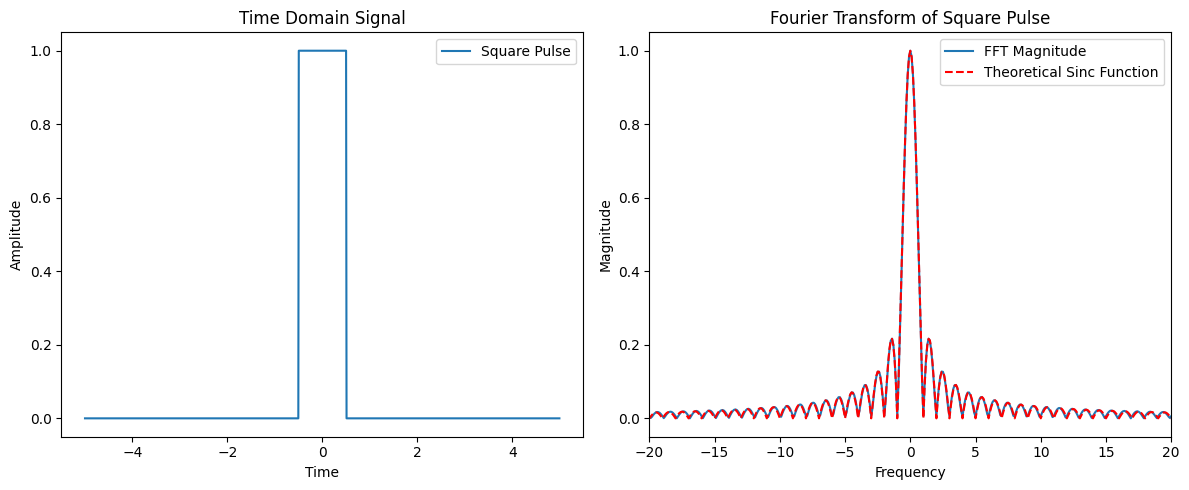
\includegraphics[width=0.9\linewidth]{figures/fft_square_pulse.png}
    \caption{FFT of a square pulse using scipy.}
    \label{fig:fft_square}
\end{figure}

In Fig.\ref{fig:fft_square}, The FFT result (blue curve) shows a sinc function, which matches the theoretical result (red dashed line).
The width of the main lobe is inversely proportional to T (the pulse width), demonstrating the duality between time and frequency: the wider the time domain signal, the narrower the frequency domain response.

\subsection{Reciprocal Space}
\hfill

\textbf{Reciprocal space} is a concept in physics and materials science, commonly found in fields such as solid-state physics, X-ray diffraction, electron diffraction, and crystallography. It forms a dual relationship with real space and is used to describe wave vectors (such as light waves, electron waves, or sound waves) within a crystal.
Definition:
Reciprocal space is a mathematical space obtained from real space (the physical space of a crystal lattice) through a Fourier transform. In reciprocal space, the periodicity of a crystal is represented by the wavenumber (k) or reciprocal lattice vector ($\mathbf{G}$), which are inversely related to the lattice constants in real space.

If the lattice in real space has basis vectors $\mathbf{a_1}$, $\mathbf{a_2}$, $\mathbf{a_3}$, then the corresponding reciprocal lattice basis vectors $\mathbf{b_1}$, $\mathbf{b_2}$, $\mathbf{b_3}$ are determined by the following relationships:
\begin{equation}
    \mathbf{b_1} = 2\pi \frac{\mathbf{a_2}\times \mathbf{a_3}}{\mathbf{a_1}\cdot(\mathbf{a_2}\times \mathbf{a_3})}
\end{equation}
\begin{equation}
    \mathbf{b_2} = 2\pi \frac{\mathbf{a_3}\times \mathbf{a_1}}{\mathbf{a_2}\cdot(\mathbf{a_3}\times \mathbf{a_1})}
\end{equation}
\begin{equation}
    \mathbf{b_3} = 2\pi \frac{\mathbf{a_1}\times \mathbf{a_2}}{\mathbf{a_3}\cdot(\mathbf{a_1}\times \mathbf{a_2})}
\end{equation}

These reciprocal lattice basis vectors satisfy the following relationship:
\begin{equation}
    \mathbf{a_i}\cdot\mathbf{b_j} = 2\pi\delta_{ij}
\end{equation}

Physical significance:
\begin{itemize}
    \item \textbf{X-ray Diffraction:}\\
    Reciprocal space describes the Fourier components of a crystal structure. The Bragg diffraction condition is often expressed in reciprocal space as:
    \begin{equation}
        \mathbf{k^\prime}-\mathbf{k} =\mathbf{G}
    \end{equation}
    where $\mathbf{k}$ and $\mathbf{k^\prime}$ are the wave vectors of the incident and scattered light, respectively, and $\mathbf{G}$ is the reciprocal lattice vector.
    \item \textbf{Electronic Band Structure:}
    In solid-state physics, the wave nature of electrons is closely related to reciprocal space through Bloch's theorem. Band structure diagrams are often plotted in reciprocal space.
    \item \textbf{Fourier Transform:}\\
    The electron density and atomic arrangement of materials can be transformed into reciprocal space using Fourier transforms, facilitating spectral analysis.
\end{itemize}

\subsection{Diffraction and interference}
\hfill

\begin{itemize}
    \item \textbf{Diffraction:}\\
    The bending and spreading of waves when they encounter an obstacle or pass through a narrow opening.
    \item \textbf{Interference:}\\
    The overlapping of two or more waves leads to constructive or destructive patterns.
    \item \textbf{Single-Slit Diffraction Pattern:}\\
    The intensity distribution follows a $sinc^2$ function:
    \begin{equation}
    I(\theta) = I_0 \left( \frac{\sin \left( \pi a \sin \theta/\lambda \right)}{\pi a \sin \theta/\lambda} \right)^2 = I_0 sinc^2(\pi a \sin \theta/\lambda)
    \end{equation}
    This pattern closely resembles the Fourier transform of a square pulse, which is also a sinc function. This is because the single-slit aperture acts as a spatial filter, and its diffraction pattern is its Fourier transform.
    \begin{figure}[h]
        \centering
        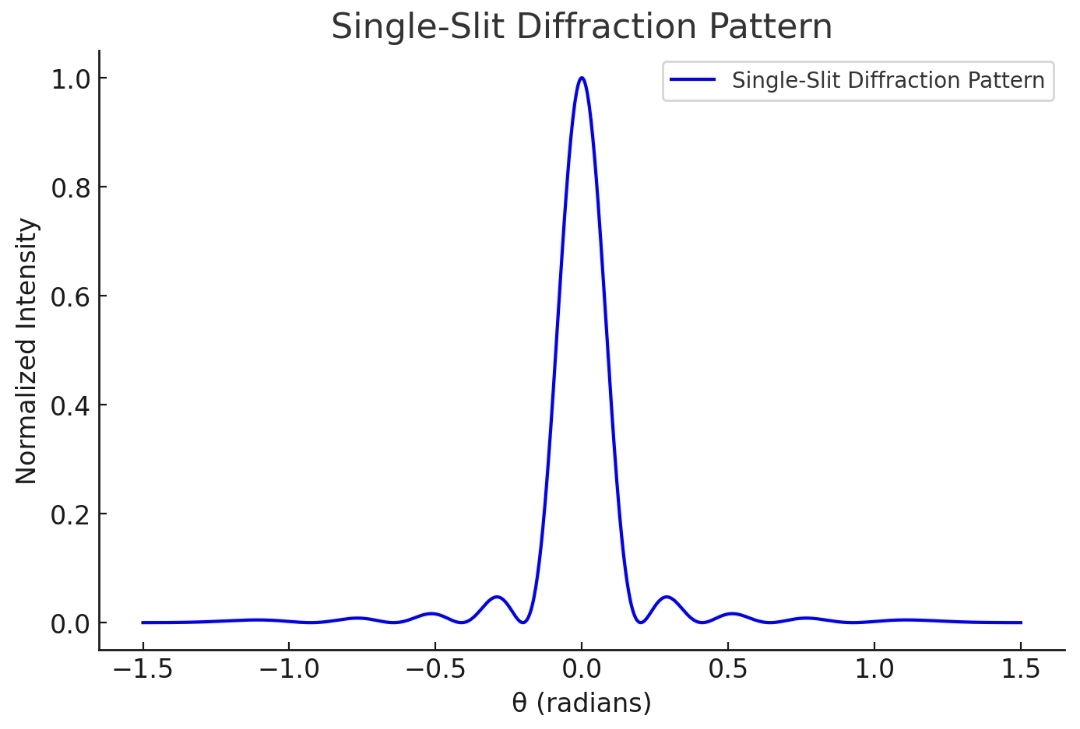
\includegraphics[width=0.8\linewidth]{figures/Single-Slit_Diffraction_Pattern.jpg}
        \caption{Single-slit diffraction pattern}
        \label{fig:single-slit}
    \end{figure}
\end{itemize}


\clearpage
\section{Experimental steps}

\subsection{Graphene Crystal Structure}
% \hfill

\begin{enumerate}
    \item \textbf{Describe the type of lattice present in graphene.}
    \item \textbf{Identify the basis atoms in the unit cell of graphene.}
    \item \textbf{How many carbon atoms constitute the basis?}
    \item \textbf{Express the lattice vectors.}
    \item \textbf{Use these vectors to generate graphene lattice via Python.}
\end{enumerate}
\textbf{Bonus:}
\begin{enumerate}
    \item \textbf{Use MATLAB/Python to create a twisted bilayer graphene Moiré pattern (in real space).}
    \item \textbf{Find the relationship between the periodicity of the Moiré pattern and its twist angles.}
\end{enumerate}

% \clearpage
\subsection{Reciprocal Space}
% \hfill

\begin{enumerate}
    \item \textbf{Please draw the reciprocal lattice vector G in Fig.\ref{fig:demon_reciprocal}(b) and define the length of G.}
    \begin{figure}[h]
        \centering
        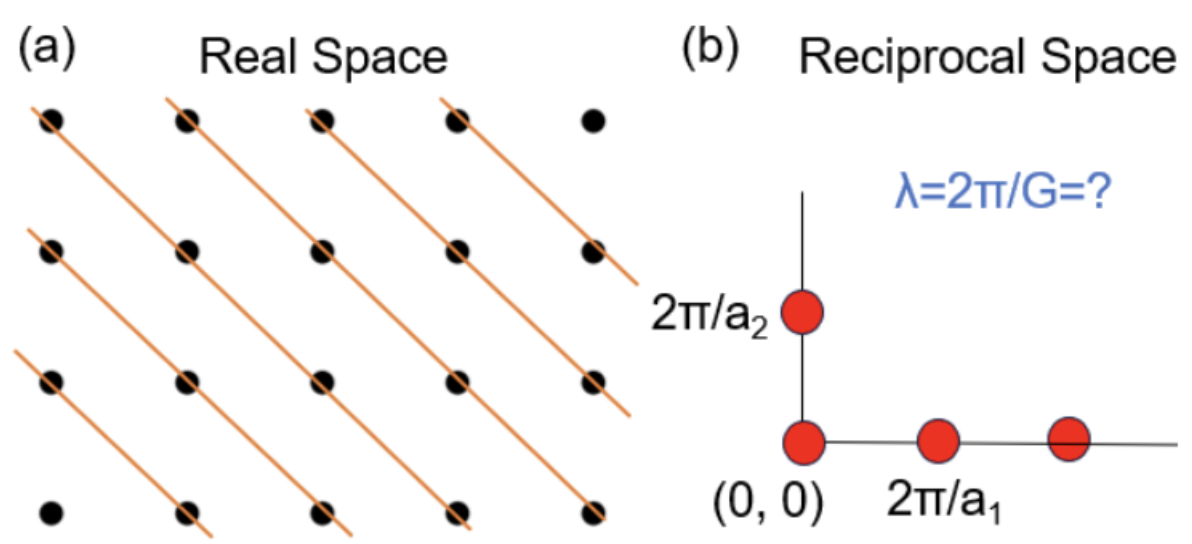
\includegraphics[width=0.5\linewidth]{figures/reciprocal.png}
        \caption{Demonstration of reciprocal space (credit: Experiment Guideline)}
        \label{fig:demon_reciprocal}
    \end{figure}
    \item \textbf{Use the relationship ($\mathbf{b_i \cdot a_i} =2\pi \delta_{ij}$ where $\delta_{ij}=1$ if $i=j$ and $\delta_{ij}=0$ if $i\neq j$) to obtain the reciprocal lattice vectors of graphene and again use python to generate the reciprocal lattice point of graphene. Find the diffraction patterns of graphene from a website and define the reciprocal lattice vectors. Compare these obtained vectors with your results.}
    \item \textbf{Use the lattice points and the reciprocal lattice vectors you obtained from Python to check if reciprocal lattice points can be mapped out by the set of reciprocal lattice vectors that yield plane waves with the periodicity of a given Bravais lattice.}
\end{enumerate}

\clearpage
\section{Result}\label{sec:result}

\subsection{Graphene Crystal Structure}\label{subsec:result_graphene}

\begin{enumerate}
    \item \textbf{Describe the type of lattice present in graphene.}\\
    Graphene has a honeycomb lattice structure, which can be described as a hexagonal (2D) Bravais lattice with a two-atom basis. The underlying lattice is a triangular Bravais lattice, but the honeycomb structure emerges due to the presence of two inequivalent carbon atoms (A and B) in each unit cell.
    \item \textbf{Identify the basis atoms in the unit cell of graphene.}\\
    Graphene's unit cell consists of two carbon atoms, labeled as A and B.
    \begin{itemize}
        \item \textbf{Atom A:} Located at $\left(0, 0\right)$
        \item \textbf{Atom B:} Located at $\left(\frac{a}{2}, \frac{\sqrt{3}a}{6}\right)$, where $a$ is the nearest-neighbor bond length
    \end{itemize}

    \item \textbf{How many carbon atoms constitute the basis?}\\
    The basis of graphene consists of two carbon atoms per unit cell.
    \item \textbf{Express the lattice vectors.}\\
    Graphene's \textbf{primitive lattice vectors} ($a_1$ and $a_2$) in Cartesian coordinates are:
    \begin{equation}
        \mathbf{a_{1}}=\left( \frac{3a}{2}, \frac{\sqrt{3}a}{2}\right)
    \end{equation}
    \begin{equation}
        \mathbf{a_{2}}=\left( \frac{3a}{2}, -\frac{\sqrt{3}a}{2}\right)
    \end{equation}
    where $a$ is the \textbf{nearest-neighbor bond length} (approximately 1.42\AA), and the \textbf{lattice constant} $a_0$ (distance between two adjacent unit cells) is given by:
    \begin{equation}
        a_{0} = \sqrt{3}a \approx 2.46 \textit{\AA}
    \end{equation}
    \begin{figure}[h]
        \centering
        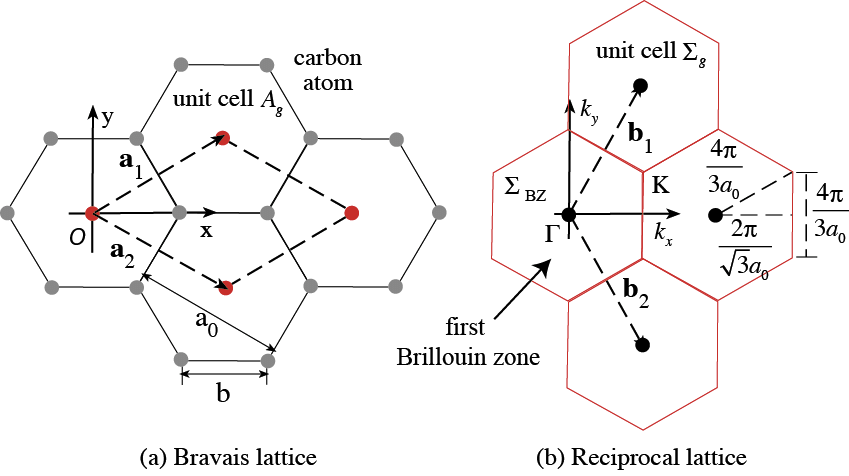
\includegraphics[width=0.5\linewidth]{figures/graphene_lattice.png}
        \caption{The structure of graphene. (a) Bravais lattice; (b) reciprocal lattice. [1]}
        \label{fig:graphene_lattice_cartoon}
    \end{figure}
    \clearpage
    \item \textbf{Use these vectors to generate graphene lattice via Python.}
    \begin{figure}[h]
        \centering
        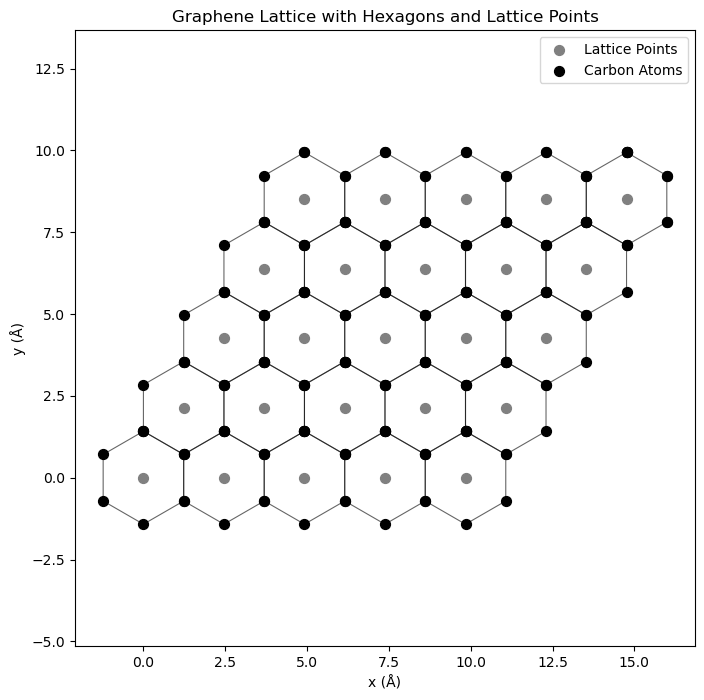
\includegraphics[width=0.6\linewidth]{figures/graphene.png}
        \caption{Lattice points of graphene}
        \label{fig:graphene_lattice}
    \end{figure}    
\end{enumerate}

% \clearpage
\textbf{Bonus:}
\begin{enumerate}
    \item \textbf{Use MATLAB/Python to create a twisted bilayer graphene Moiré pattern (in real space).}
    \begin{itemize}
        \item 1$^\circ$
    \end{itemize}
    \begin{figure}[h]
        \centering
        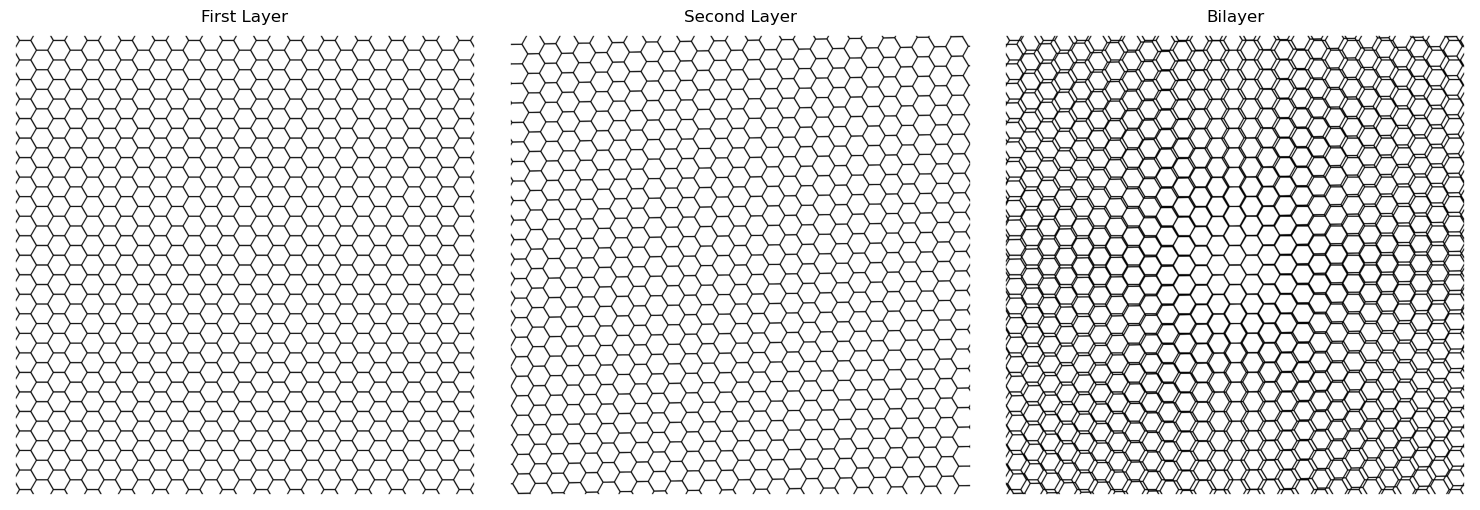
\includegraphics[width=0.82\linewidth]{figures/1degree.png}
        \caption{A twisted bilayer graphene Moiré pattern (1$^\circ$)}
        \label{fig:moire_1}
    \end{figure}
    \clearpage
    \item 5$^\circ$
    \begin{figure}[h]
        \centering
        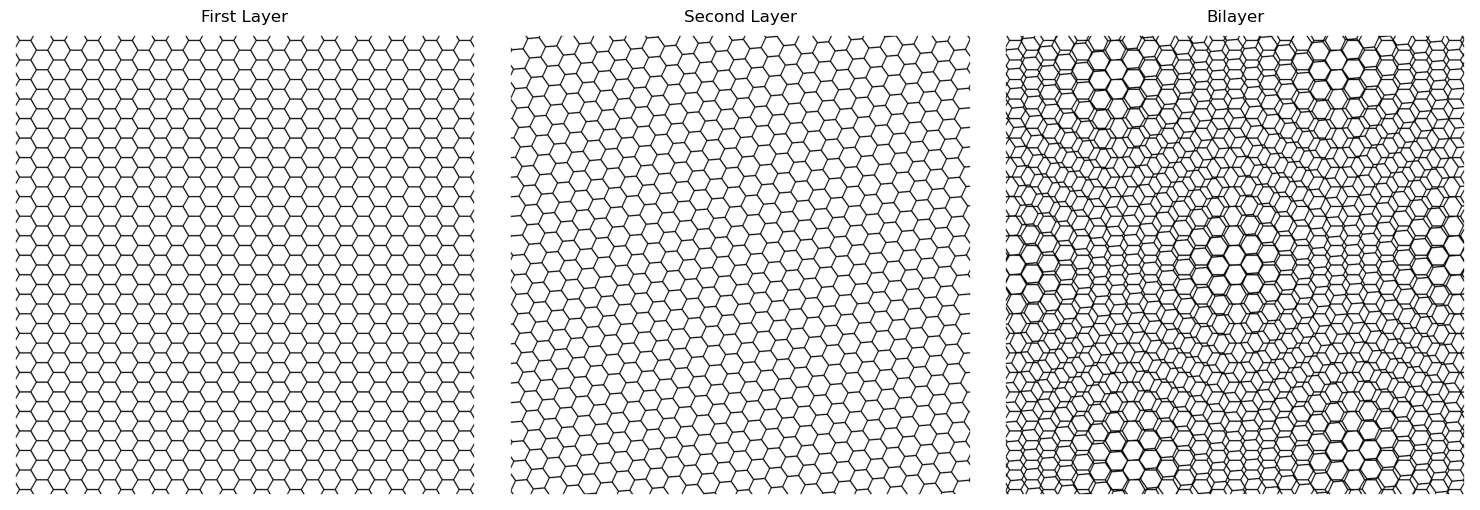
\includegraphics[width=0.82\linewidth]{figures/5degree.png}
        \caption{\textit{continued} (5$^\circ$)}
        \label{fig:moire_5}
    \end{figure}
    \item 10$^\circ$
    \begin{figure}[h]
        \centering
        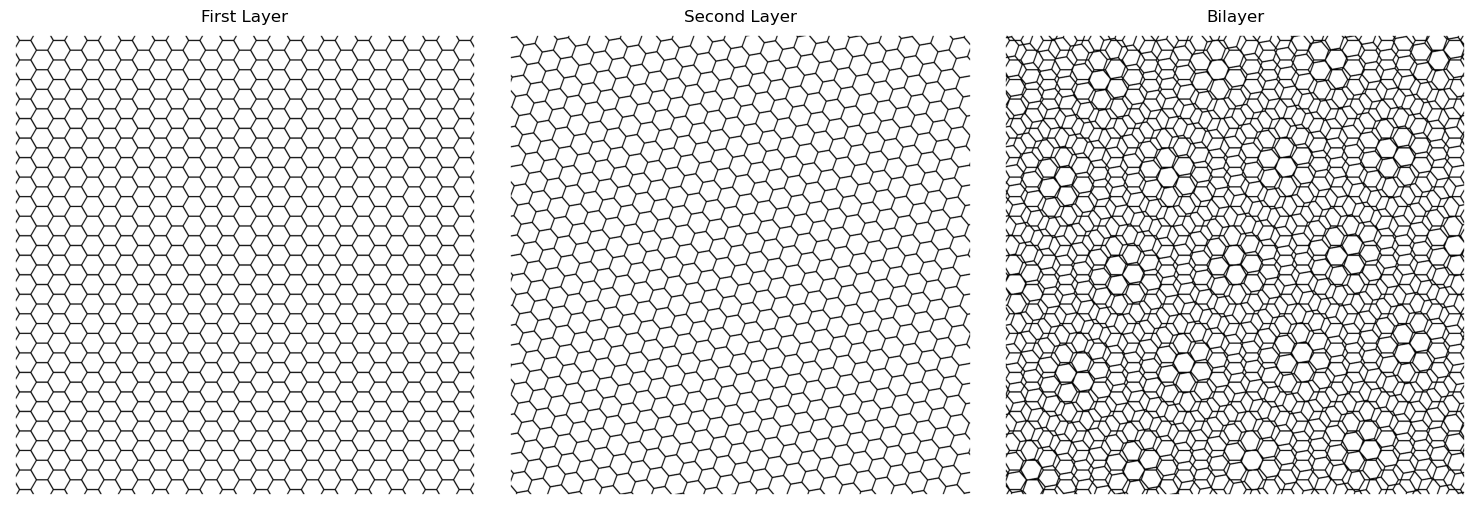
\includegraphics[width=0.82\linewidth]{figures/10degree.png}
        \caption{\textit{continued} (10$^\circ$)}
        \label{fig:moire_10}
    \end{figure}
    
    \begin{itemize}
        \item 15$^\circ$
    \end{itemize}
    \begin{figure}[h]
        \centering
        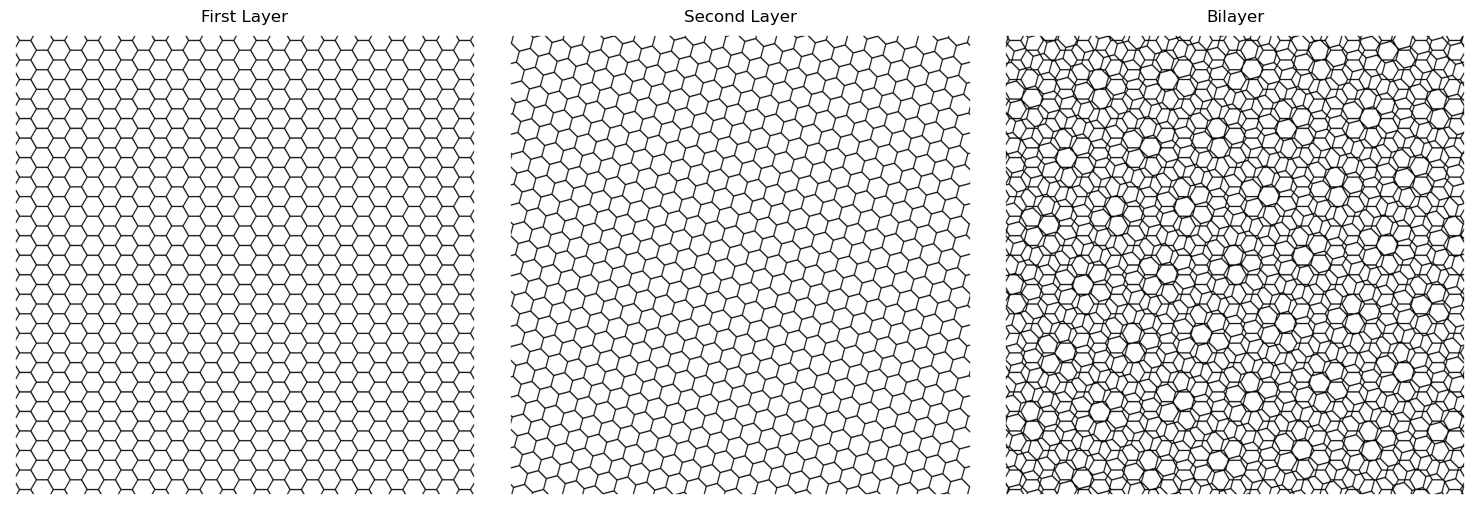
\includegraphics[width=0.82\linewidth]{figures/15degree.png}
        \caption{\textit{continued} (15$^\circ$)}
        \label{fig:moire_15}
    \end{figure}
    \clearpage
    \item 20$^\circ$
    \begin{figure}[h]
        \centering
        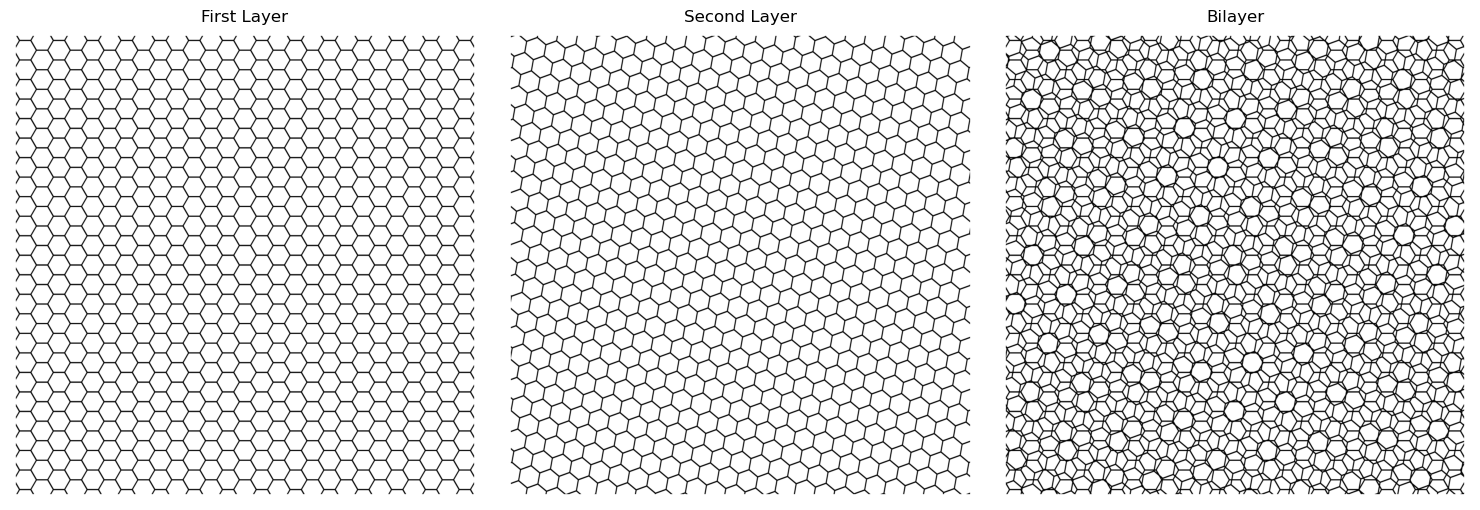
\includegraphics[width=0.82\linewidth]{figures/20degree.png}
        \caption{\textit{continued} (20$^\circ$)}
        \label{fig:moire_20}
    \end{figure}
    \item 30$^\circ$
    \begin{figure}[h]
        \centering
        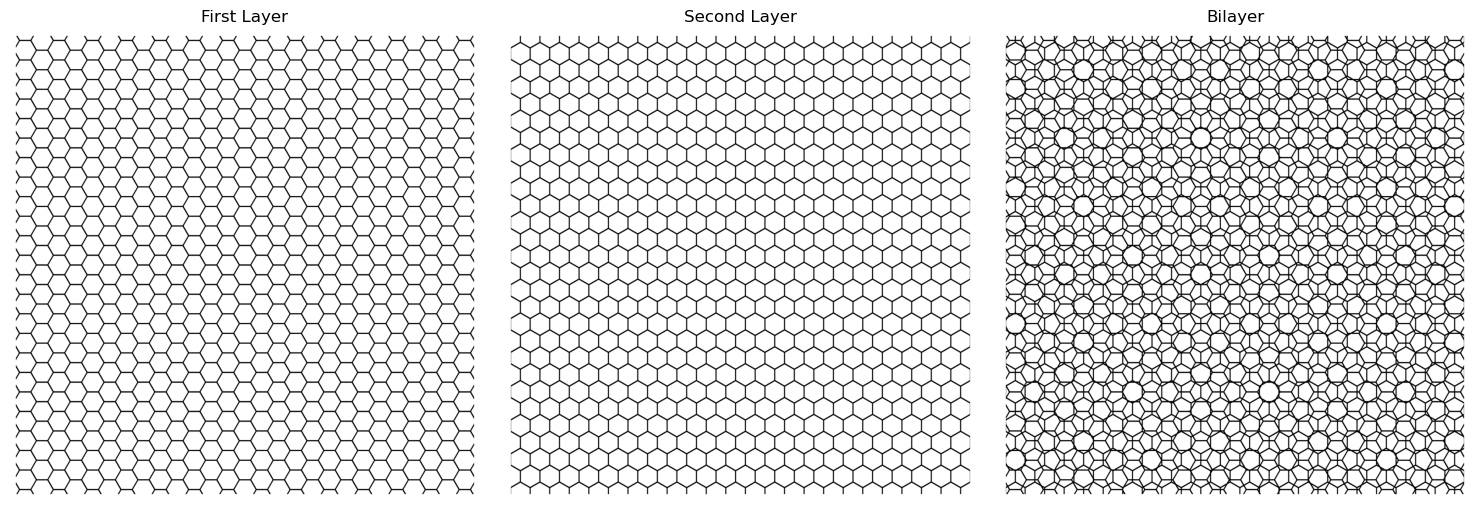
\includegraphics[width=0.82\linewidth]{figures/30degree.png}
        \caption{\textit{continued} (30$^\circ$)}
        \label{fig:moire_30}
    \end{figure}
    
    \begin{itemize}
        \item 45$^\circ$
    \end{itemize}
    \begin{figure}[h]
        \centering
        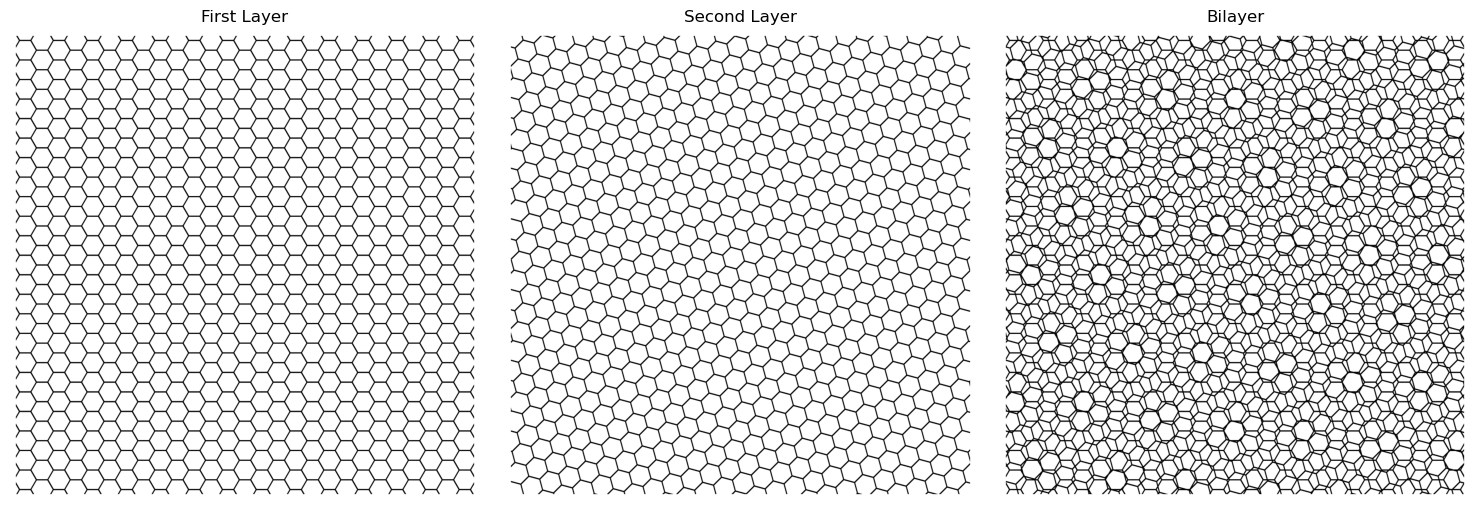
\includegraphics[width=0.82\linewidth]{figures/45degree.png}
        \caption{\textit{continued} (45$^\circ$)}
        \label{fig:moire_45}
    \end{figure}
    \clearpage
    \item 60$^\circ$
    \begin{figure}[h]
        \centering
        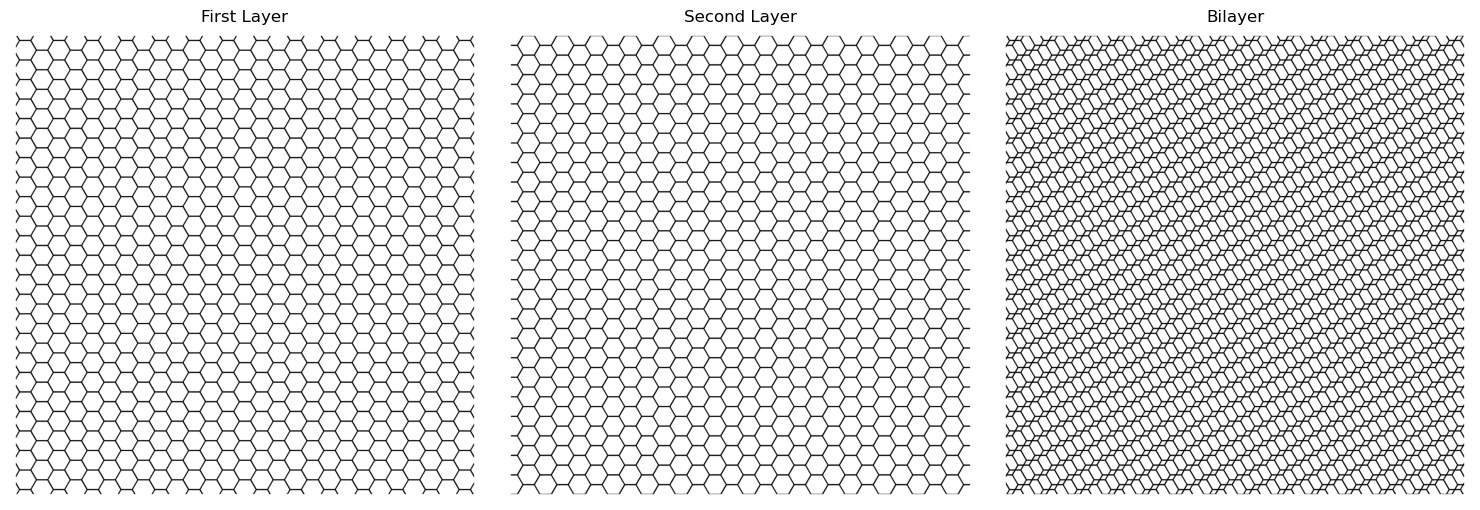
\includegraphics[width=0.82\linewidth]{figures/60degree.png}
        \caption{\textit{continued} (60$^\circ$)}
        \label{fig:moire_60}
    \end{figure}
    \item 75$^\circ$
    \begin{figure}[h]
        \centering
        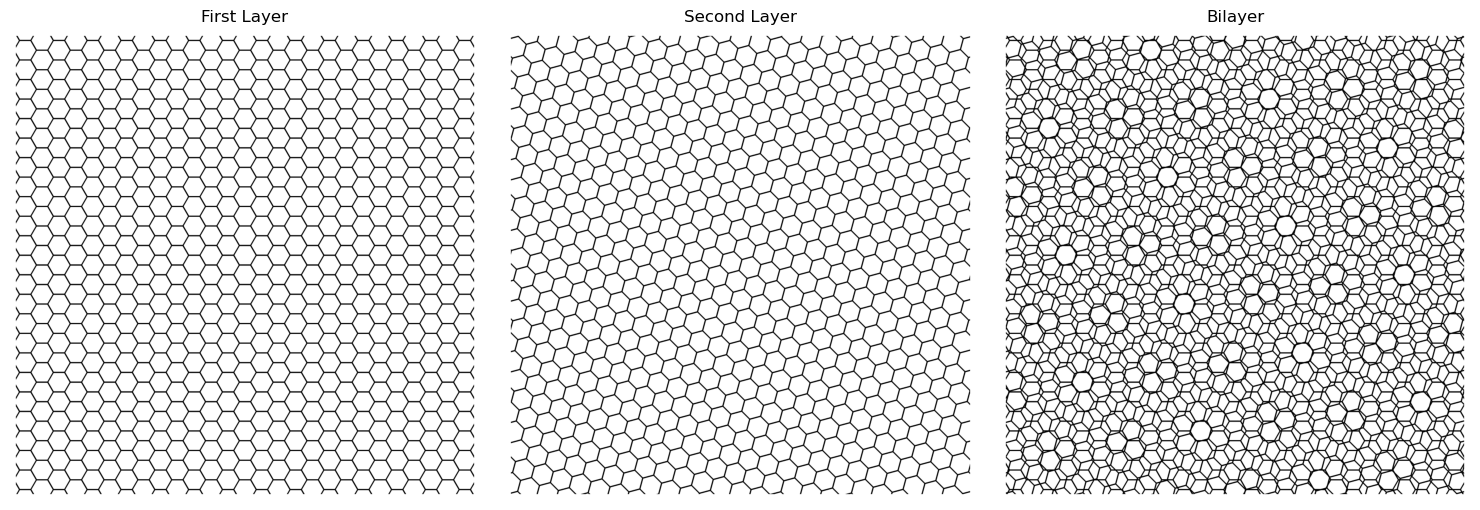
\includegraphics[width=0.82\linewidth]{figures/75degree.png}
        \caption{\textit{continued} 75$^\circ$)}
        \label{fig:moire_75}
    \end{figure}
    \begin{figure}[h]
        \centering
        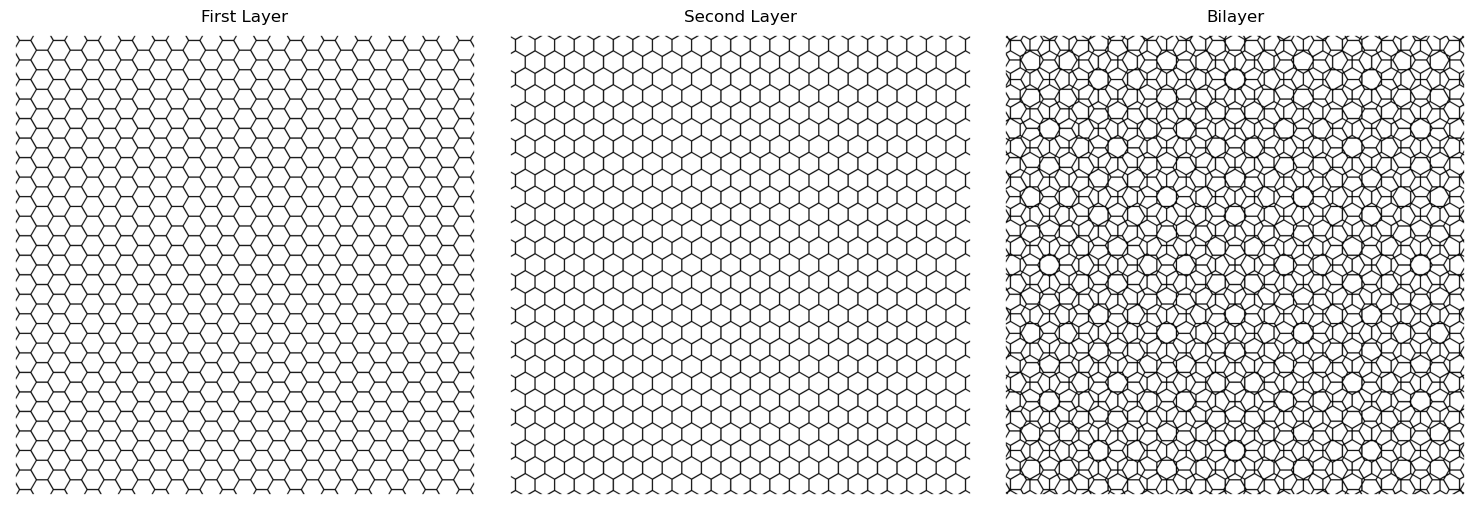
\includegraphics[width=0.82\linewidth]{figures/90degree.png}
        \caption{\textit{continued} (90$^\circ$)}
        \label{fig:moire_90}
    \end{figure}
    \clearpage
    \item \textbf{Find the relationship between the periodicity of the Moiré pattern and its twist angles.}\\
    When the lattice constant of the two layers of graphene ($a_0$, approximately 2.46 \AA) and their twist angle (θ, assuming θ is very small) are given, the Moiré pattern periodicity L can be approximated as:
    \begin{equation}
    \label{eq:moire}
        L\approx \frac{a_0}{2sin(\theta/2)}
    \end{equation}
    where L = Moiré pattern periodicity,  $a_0$ is graphene lattice constant (approximately 2.46 Å), and θ is twist angle (in radians)
    
As the twist angle θ decreases, the Moiré pattern periodicity L increases.

(A detailed analysis is in the Sec. \ref{subsec:discussion_graphene}.)
\end{enumerate}

% \clearpage
\subsection{Reciprocal Space}

\begin{enumerate}
    \item \textbf{Please draw the reciprocal lattice vector G in Fig.\ref{fig:demon_reciprocal}(b) and define the length of G.}\\
    (There are a few corrections from the experiment notebook, e.g., Fig. 7 in the notebook.)\\   
    The \textbf{reciprocal lattice vector}:
    \begin{equation}
        \mathbf{G} = \frac{2\pi}{a_1}\mathbf{\hat{i}}+\frac{2\pi}{a_2}\mathbf{\hat{j}}
    \end{equation}
    \begin{equation}
        |\mathbf{G}| = 2\pi \sqrt{\left(\frac{1}{a_1}\right)^2+\left(\frac{1}{a_2}\right)^2}
    \end{equation}
    The \textbf{wavelength}:
    \begin{equation}
        \lambda = \frac{2\pi}{|\mathbf{G}|} = \frac{1}{\sqrt{\left(\frac{1}{a_1}\right)^2+\left(\frac{1}{a_2}\right)^2}}
    \end{equation}
    % \clearpage
    \item \textbf{Use the relationship ($\mathbf{b_i \cdot a_i} =2\pi \delta_{ij}$ where $\delta_{ij}=1$ if $i=j$ and $\delta_{ij}=0$ if $i\neq j$) to obtain the reciprocal lattice vectors of graphene and again use python to generate the reciprocal lattice point of graphene. Find the diffraction patterns of graphene from a website and define the reciprocal lattice vectors. Compare these obtained vectors with your results.}
    \begin{enumerate}
        \item \textbf{Use Python to generate the reciprocal lattice of graphene and calculate its $\mathbf{b_1}$ and $\mathbf{b_2}$:}
        \begin{enumerate}
            \item This part simulates the honeycomb lattice of graphene, where the angle between the two basis vectors is 120$^{\circ}$. The basis vectors, $a_1$ and $a_2$ form the lattice vectors in real space.
            \begin{equation}
                \mathbf{a_1} = \left(0, 0\right)
            \end{equation}
            \begin{equation}
                \mathbf{a_2} = a\cdot\left(cos(120^\circ), sin(120^\circ)\right) = \left(-\frac{a}{2}, \frac{\sqrt{3}a}{2}\right)
            \end{equation}
            \clearpage
            \begin{figure}[h]
                \centering
                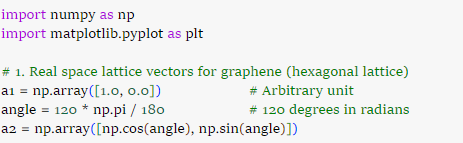
\includegraphics[width=0.7\linewidth]{figures/result_2_2_1.png}
                \caption{Real Space Lattice Vectors}
                \label{fig:result_2_2_1}
            \end{figure}
            
            \item We use the cross product of vectors to determine the reciprocal lattice, which must be handled in three-dimensional space.
            \begin{figure}[h]
                \centering
                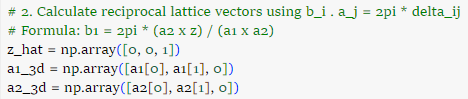
\includegraphics[width=0.7\linewidth]{figures/result_2_2_2.png}
                \caption{Reciprocal Lattice Vectors}
                \label{fig:result_2_2_2}
            \end{figure}
            \item According to the definition, i.e., $\mathbf{b_i \cdot a_i} =2\pi \delta_{ij}$, the reciprocal lattice vectors are determined as following:
            \begin{equation}
                \mathbf{b_1} = \frac{2\pi (\mathbf{\hat{z}}\times \mathbf{a_2})}{|\mathbf{a_1}\times \mathbf{a_2}|} = \left(\frac{2\pi}{a}, \frac{2\pi}{\sqrt{3}a}\right)
            \end{equation}
            \begin{equation}
                \mathbf{b_2} = \frac{2\pi (\mathbf{a_1}\times \mathbf{\hat{z}})}{|\mathbf{a_1}\times \mathbf{a_2}|} = \left(0, \frac{4\pi}{\sqrt{3}a}\right)
            \end{equation}
            \begin{figure}[h]
                \centering
                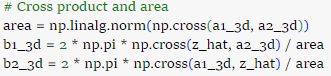
\includegraphics[width=0.7\linewidth]{figures/result_2_2_3.png}
                \caption{Cross product and area}
                \label{fig:result_2_2_3}
            \end{figure}
            \clearpage
            \item Project them back into 2D to obtain the reciprocal lattice vectors b1 and b2 for visualization.
            \begin{figure}[h]
                \centering
                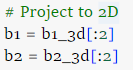
\includegraphics[width=0.3\linewidth]{figures/result_2_2_4.png}
                \caption{Project to 2D}
                \label{fig:result_2_2_4}
            \end{figure}
            % \clearpage
            \item Use a nested “for loop”  to generate all reciprocal lattice points through the linear combination “n*b1+m*b2”
            \begin{figure}[h]
                \centering
                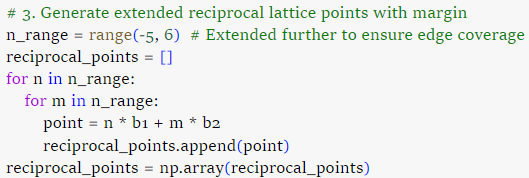
\includegraphics[width=0.7\linewidth]{figures/result_2_2_5.png}
                \caption{Reciprocal Lattice Points}
                \label{fig:result_2_2_5}
            \end{figure}
            \item Initialize the plot and draw all reciprocal lattice points, marking them with blue dots.
            \begin{figure}[h]
                \centering
                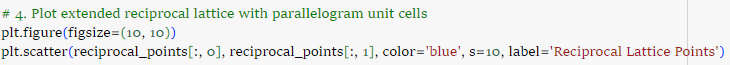
\includegraphics[width=0.7\linewidth]{figures/result_2_2_6.png}
                \caption{Plot extended reciprocal lattice with parallelogram unit cells}
                \label{fig:result_2_2_6}
            \end{figure}
            \clearpage
            \item Check whether neighboring lattice points exist to avoid drawing incomplete unit cells beyond the boundaries. Use orange dashed lines to outline the complete parallelogram unit cell.
            \begin{figure}[h]
                \centering
                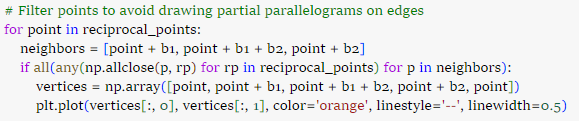
\includegraphics[width=0.6\linewidth]{figures/result_2_2_7.png}
                \caption{Filter points to avoid drawing partial parallelograms on edges}
                \label{fig:result_2_2_7}
            \end{figure}
            % \clearpage
            \item First, use arrows to indicate the reciprocal lattice vectors $\mathbf{b_1}$ and $\mathbf{b_2}$. Then, finalize the visualization by adding a title, coordinate axes, and grid lines, ensuring a consistent aspect ratio and displaying a legend.
            \begin{figure}[h]
                \centering
                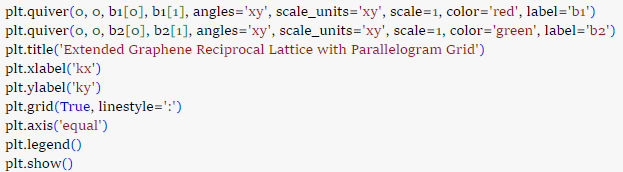
\includegraphics[width=0.7\linewidth]{figures/result_2_2_8.png}
                \caption{Refine the image for clarity and presentation}
                \label{fig:result_2_2_8}
            \end{figure}
            \begin{figure}[h]
                \centering
                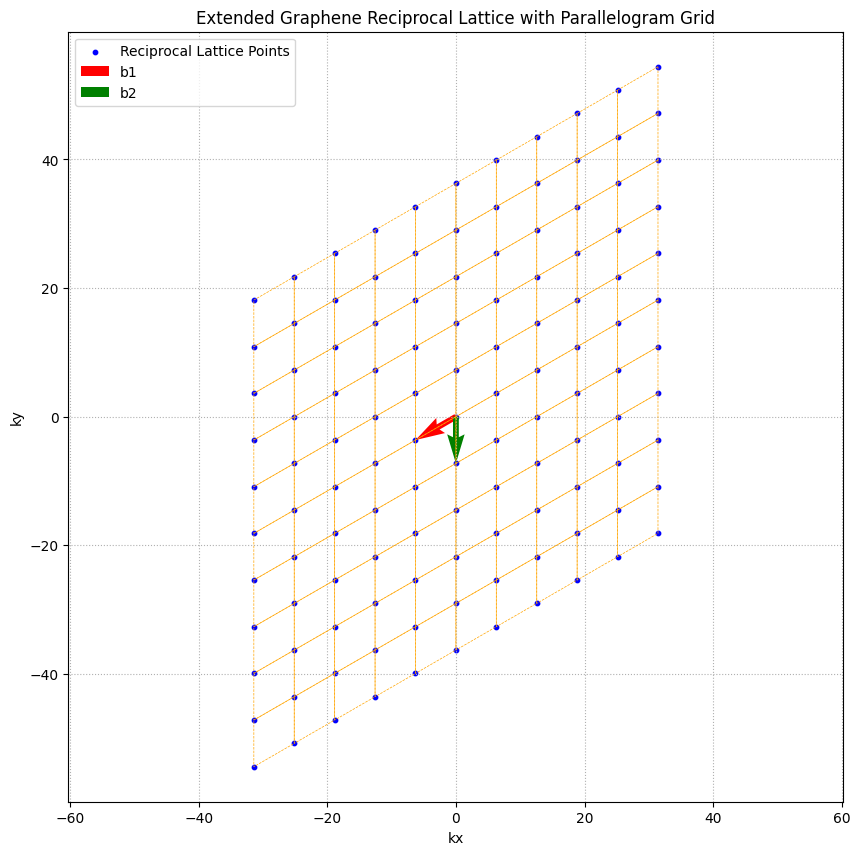
\includegraphics[width=0.5\linewidth]{figures/result_2_2_9.png}
                \caption{Reciprocal lattice of graphene}
                \label{fig:result_2_2_9}
            \end{figure}
        \end{enumerate}
        \clearpage 
        \item \textbf{Compare with the experimental diffraction pattern:}
        % \clearpage
        \begin{figure}[h]
            \centering
            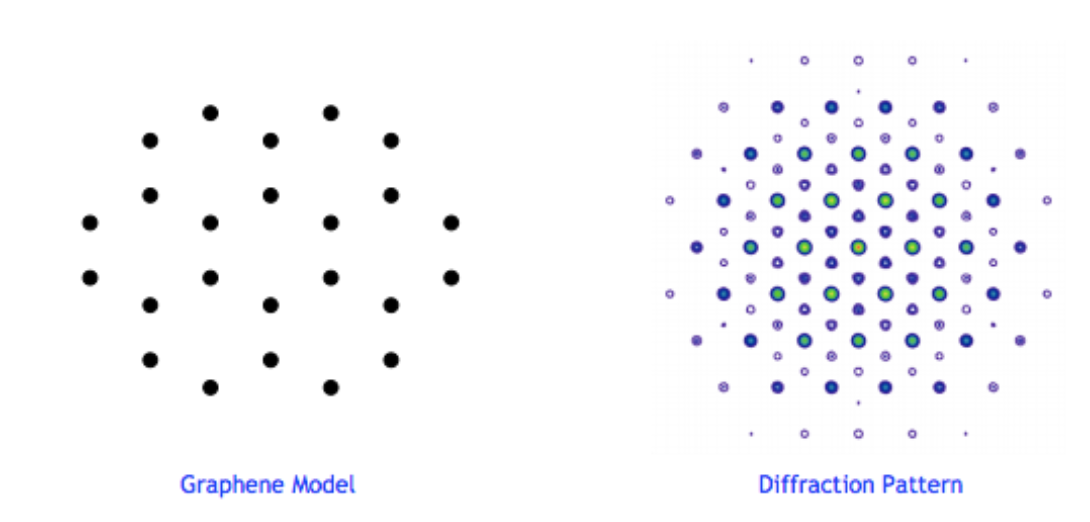
\includegraphics[width=0.4\linewidth]{figures/result_2_2_10.png}
            \caption{\textit{left}: theoretical graphene model. Black dots represent carbon atom positions, forming a hexagonal arrangement characterized by 120$^\circ$ angles and sixfold symmetry; \textit{right}: Diffraction pattern of the graphene model [2]}
            \label{fig:result_2_2_10}
        \end{figure}
        \begin{figure}[h]
            \centering
            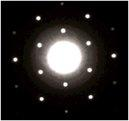
\includegraphics[width=0.15\linewidth]{figures/result_2_2_11.png}
            \caption{Graphene electron diffraction pattern [3]}
            \label{fig:result_2_2_11}
        \end{figure}
        \begin{figure}[h]
            \centering
            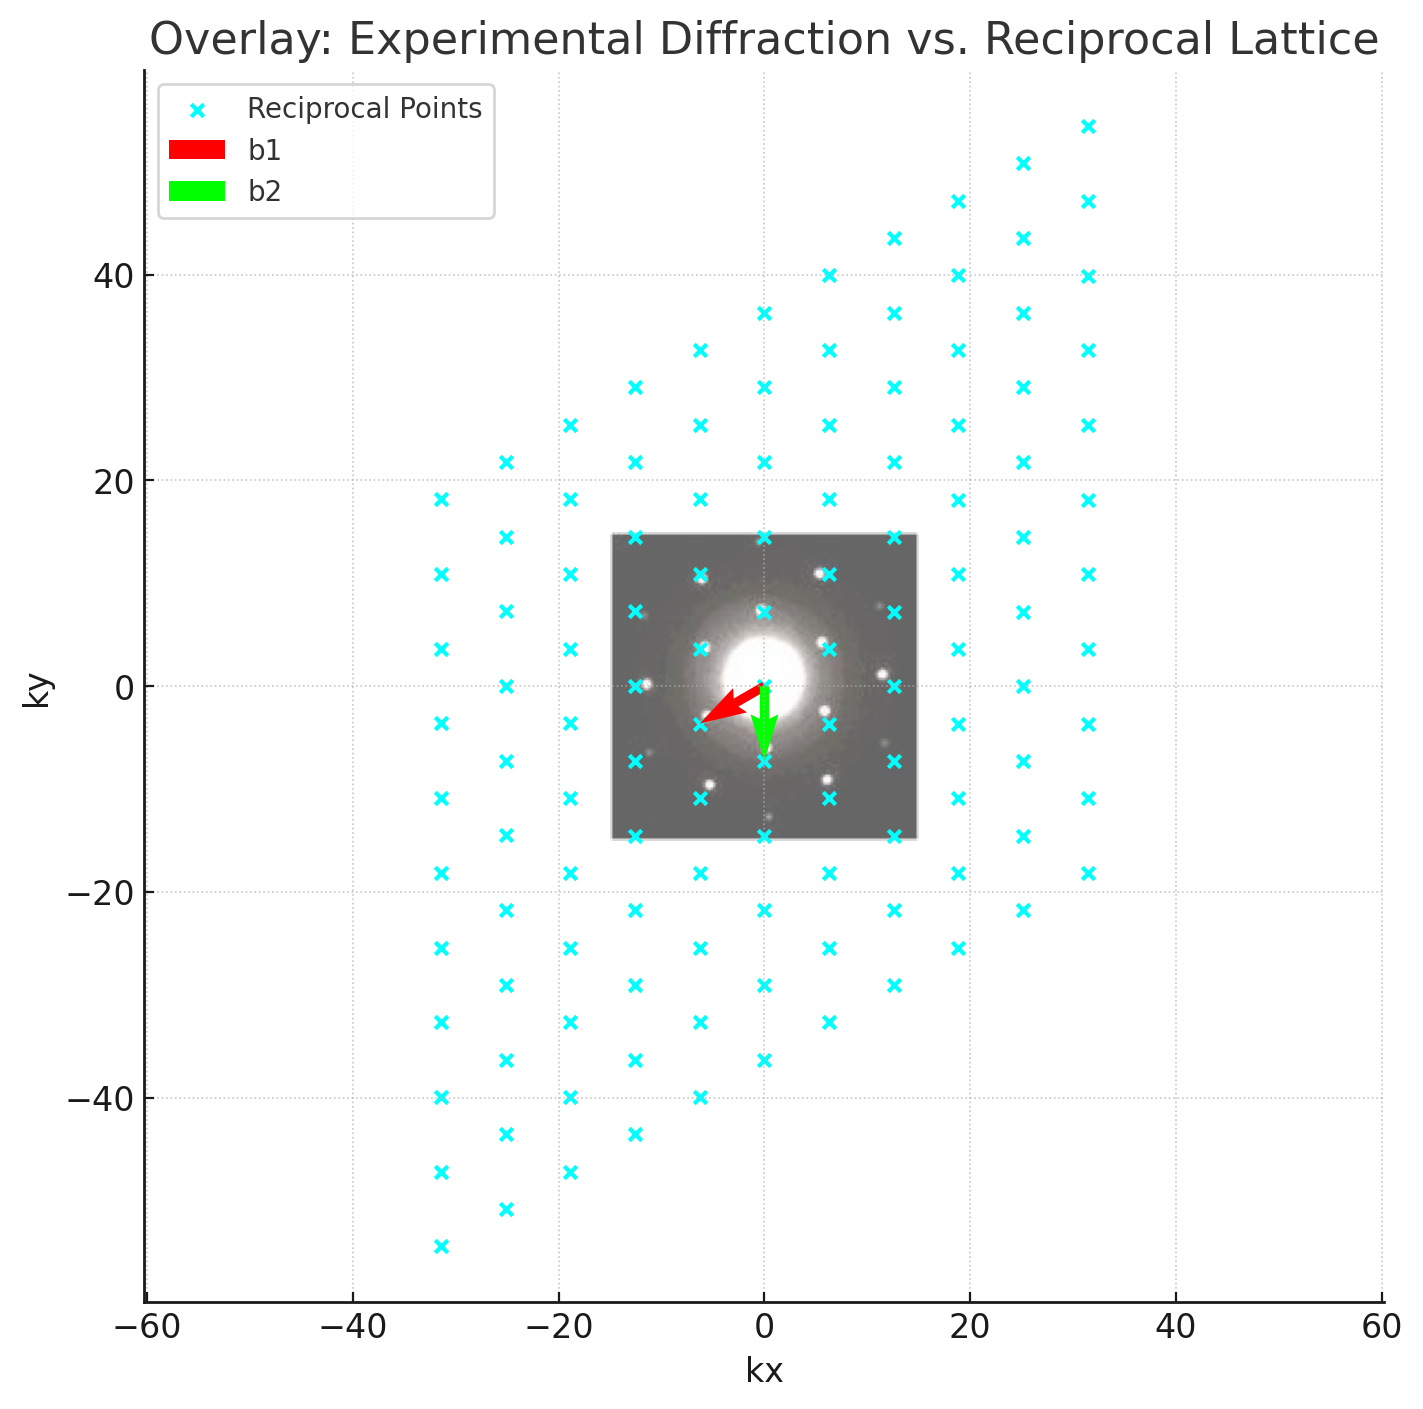
\includegraphics[width=0.5\linewidth]{figures/result_2_2_12.png}
            \vspace{-0.5cm}
            \caption{Compare the Python-generated plot with the experimental diffraction pattern}
            \label{fig:result_2_2_12}
        \end{figure}
    \end{enumerate}
    \clearpage
    \item \textbf{Use the lattice points and the reciprocal lattice vectors you obtained from Python to check if reciprocal lattice points can be mapped out by the set of reciprocal lattice vectors that yield plane waves with the periodicity of a given Bravais lattice.}\\
    The reciprocal lattice points can be generated through a linear combination:
    \begin{equation}
        \mathbf{G}_{mn} = m\mathbf{b}_1 + n\mathbf{b}_2
     \end{equation}
     where $\mathbf{G}$ is the reciprocal lattice vector. If the reciprocal lattice points can form plane waves, they must satisfy the periodicity of the Bravais lattice, which is linked to the Brillouin zone and diffraction patterns.
    \begin{itemize}
        \item In a Bravais lattice, the reciprocal lattice vectors should yield plane waves that have the same periodicity as the real-space lattice.
        \item The plane wave is given by:
        \begin{equation}
            \psi(\mathbf{r}) = e^{i \mathbf{G\cdot r}}
        \end{equation}
        where the length of $\mathbf{G}$ is $\frac{4\pi}{3a}$
        \item The reciprocal lattice vectors confirm that plane waves generated by them satisfy the periodicity of the real-space Bravais lattice.
    \end{itemize}
    (A detailed analysis is in the Sec. \ref{subsec:discussion_reciprocal}.)
\end{enumerate}



% \clearpage
\section{Analysis and Discussion}\label{sec:discussion}

\subsection{Graphene Crystal Structure}\label{subsec:discussion_graphene}

\textbf{Find the relationship between the periodicity of the Moiré pattern and its twist angles.}\\
    To estimate the periodicity of the Moiré pattern, we firstly use the FFT of the first, second, and the bilayer to ($f_{1}$, $f_{1}$, and $f_{bilaryer}$) obtain their spectra, i.e., $F_{1}$, $F_{1}$, and $F_{bilaryer}$, respectively. Then, extract the spectrum of the Moiré pattern by
    \begin{equation}
        F_{Moire} = F_{bilayer} - F_{1} - F_{2}
    \end{equation}
\begin{itemize}
    \item 1$^\circ$
    \begin{figure}[h]
        \centering
        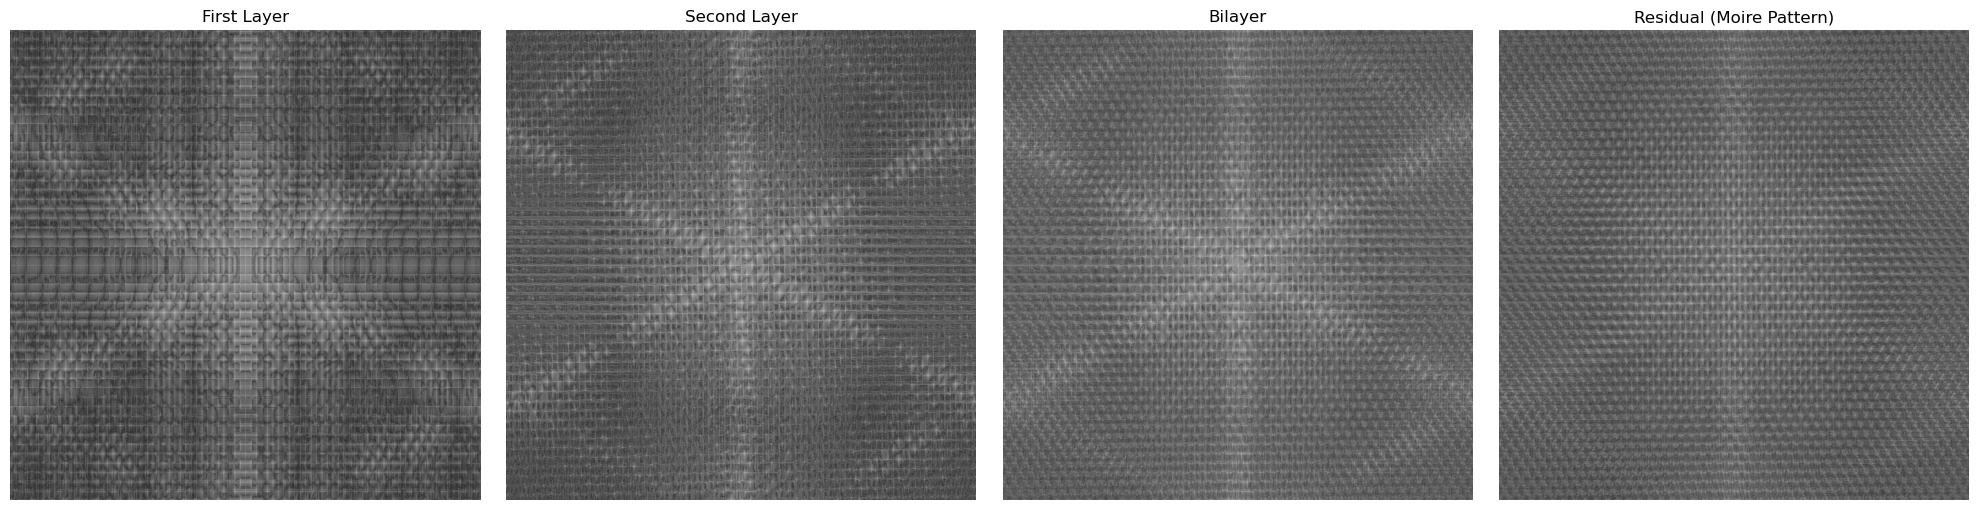
\includegraphics[width=0.95\linewidth]{figures/1degree_fft.png}
        \caption{FFT of the first (\textit{left}), second (\textit{mid-left}), and the bilayer(\textit{mid-right}). Also, we get the residual (\textit{right}), the spectrum of the Moiré pattern,  by subtracting the spectra of the bilayer from the ones of the first and second layer (1$^\circ$)}
        \label{fig:moire_1_fft}
    \end{figure}
    \clearpage
    \item 5$^\circ$
    \begin{figure}[h]
        \centering
        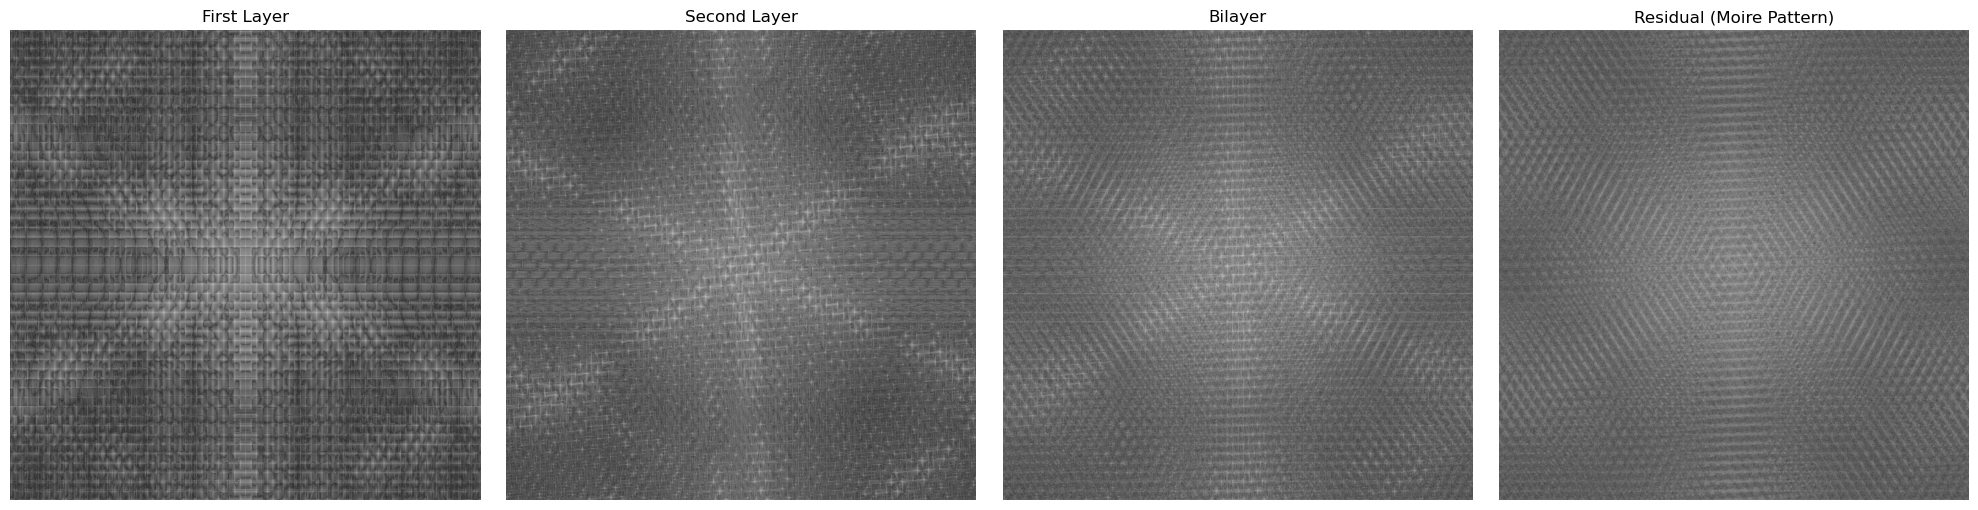
\includegraphics[width=0.95\linewidth]{figures/5degree_fft.png}
        \caption{\textit{continued} (5$^\circ$)}
        \label{fig:moire_5_fft}
    \end{figure}
    \item 10$^\circ$
    \begin{figure}[h]
        \centering
        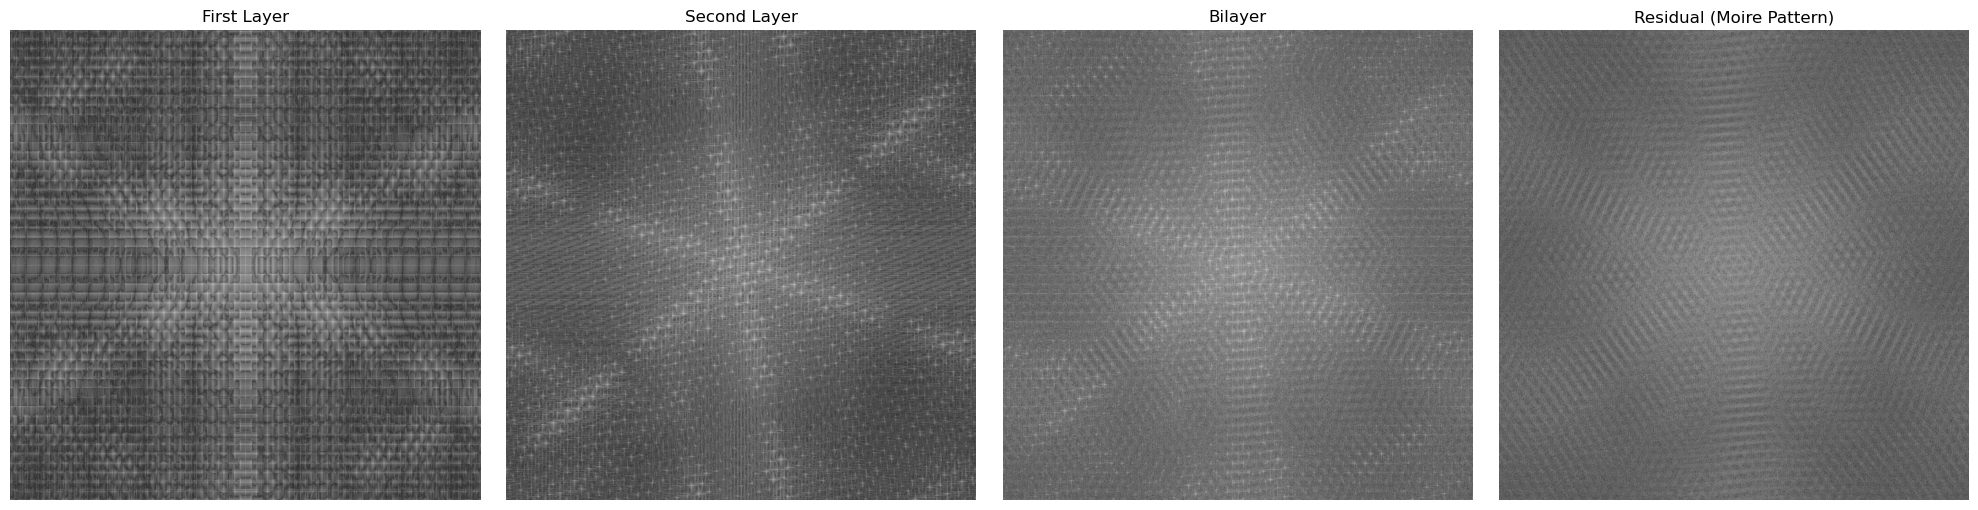
\includegraphics[width=0.95\linewidth]{figures/10degree_fft.png}
        \caption{\textit{continued} (10$^\circ$)}
        \label{fig:moire_10_fft}
    \end{figure}
    
    \item 15$^\circ$
    \begin{figure}[h]
        \centering
        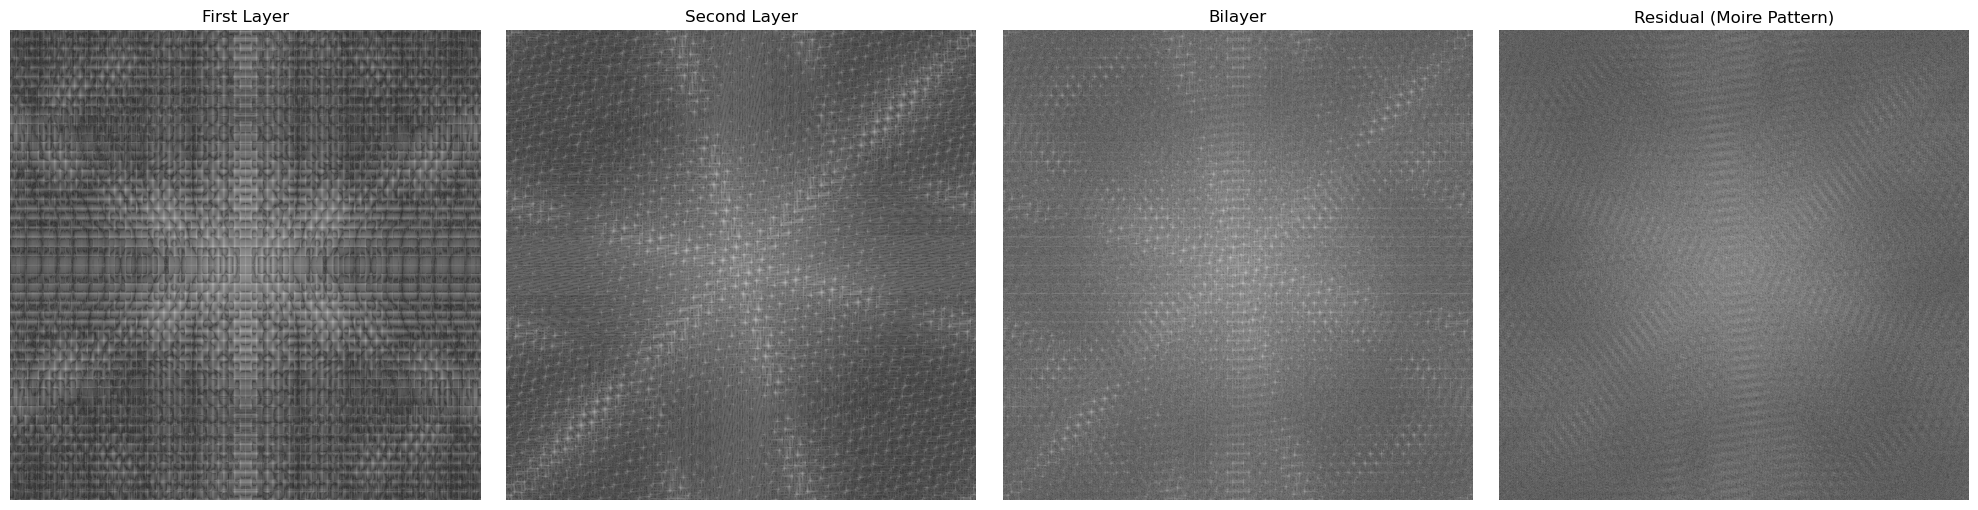
\includegraphics[width=0.95\linewidth]{figures/15degree_fft.png}
        \caption{\textit{continued} (15$^\circ$)}
        \label{fig:moire_15_fft}
    \end{figure}
    \clearpage
    \item 20$^\circ$
    \begin{figure}[h]
        \centering
        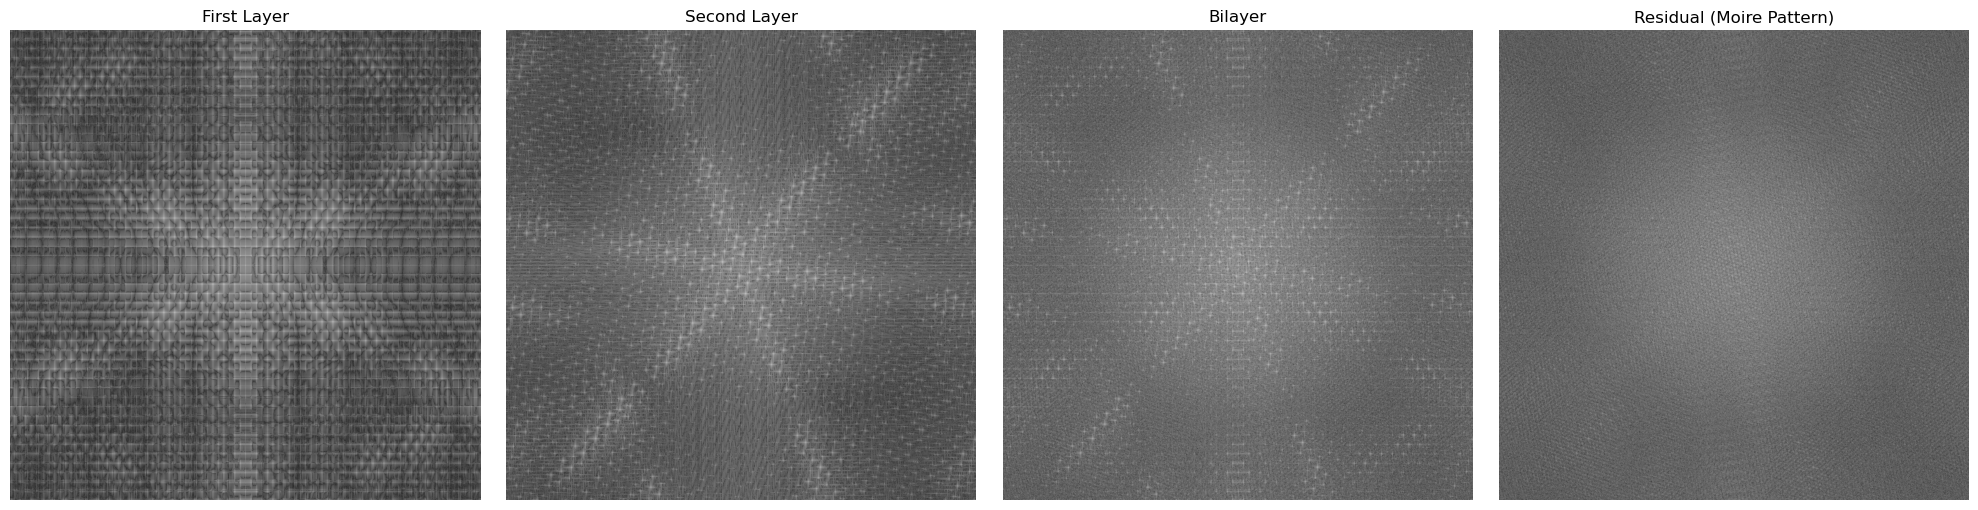
\includegraphics[width=0.95\linewidth]{figures/20degree_fft.png}
        \caption{\textit{continued} (20$^\circ$)}
        \label{fig:moire_20_fft}
    \end{figure}
    \item 30$^\circ$
    \begin{figure}[h]
        \centering
        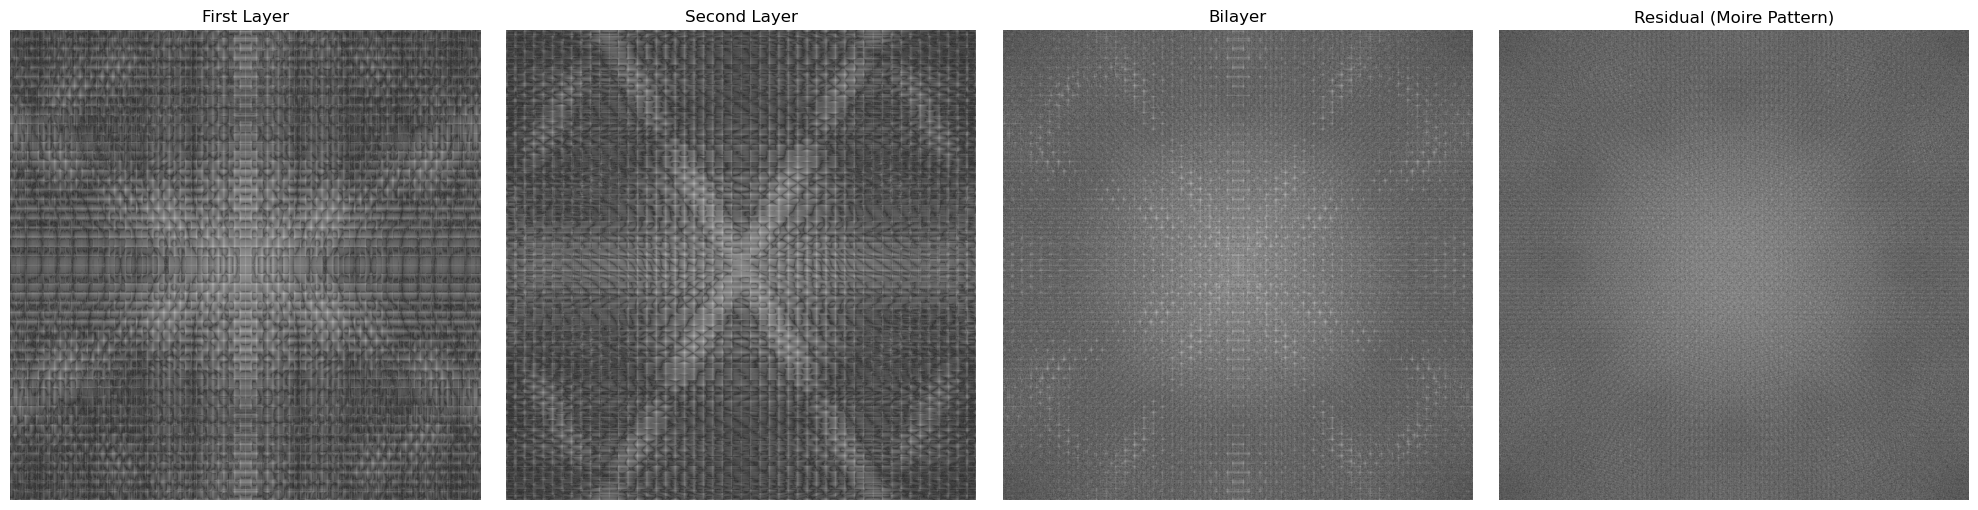
\includegraphics[width=0.95\linewidth]{figures/30degree_fft.png}
        \caption{\textit{continued} (30$^\circ$)}
        \label{fig:moire_30_fft}
    \end{figure}
    

    \item 45$^\circ$
    \begin{figure}[h]
        \centering
        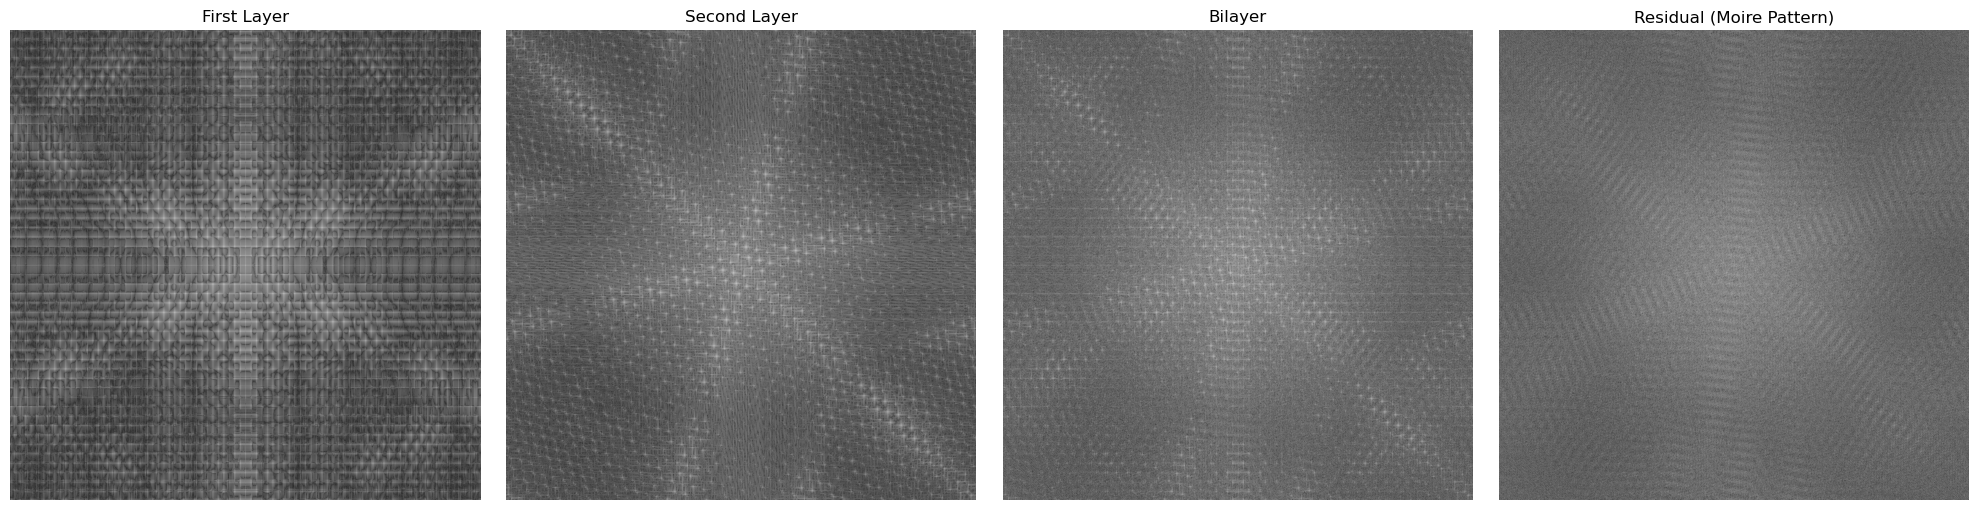
\includegraphics[width=0.95\linewidth]{figures/45degree_fft.png}
        \caption{\textit{continued} (45$^\circ$)}
        \label{fig:moire_45_fft}
    \end{figure}
    \clearpage
    \item 60$^\circ$
    \begin{figure}[h]
        \centering
        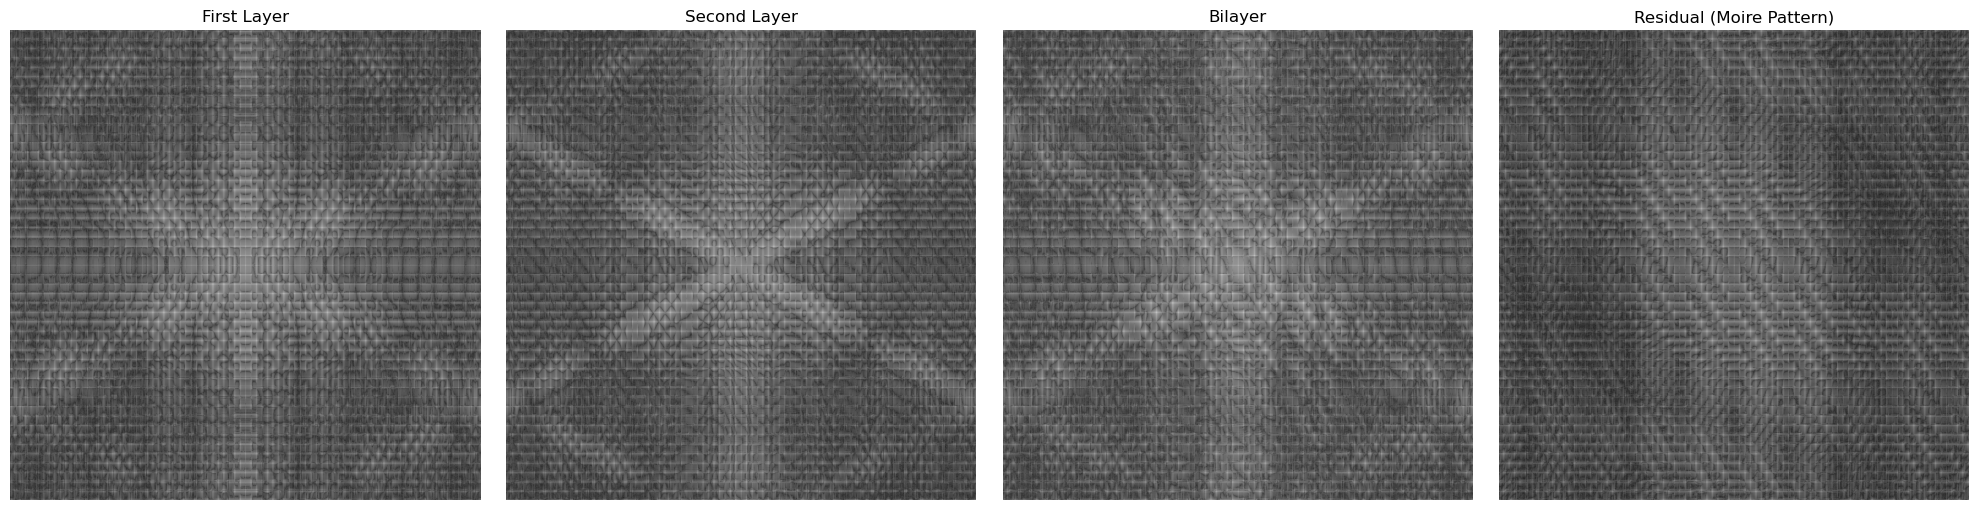
\includegraphics[width=0.95\linewidth]{figures/60degree_fft.png}
        \caption{\textit{continued} (60$^\circ$)}
        \label{fig:moire_60_fft}
    \end{figure}
    \item 75$^\circ$
    \begin{figure}[h]
        \centering
        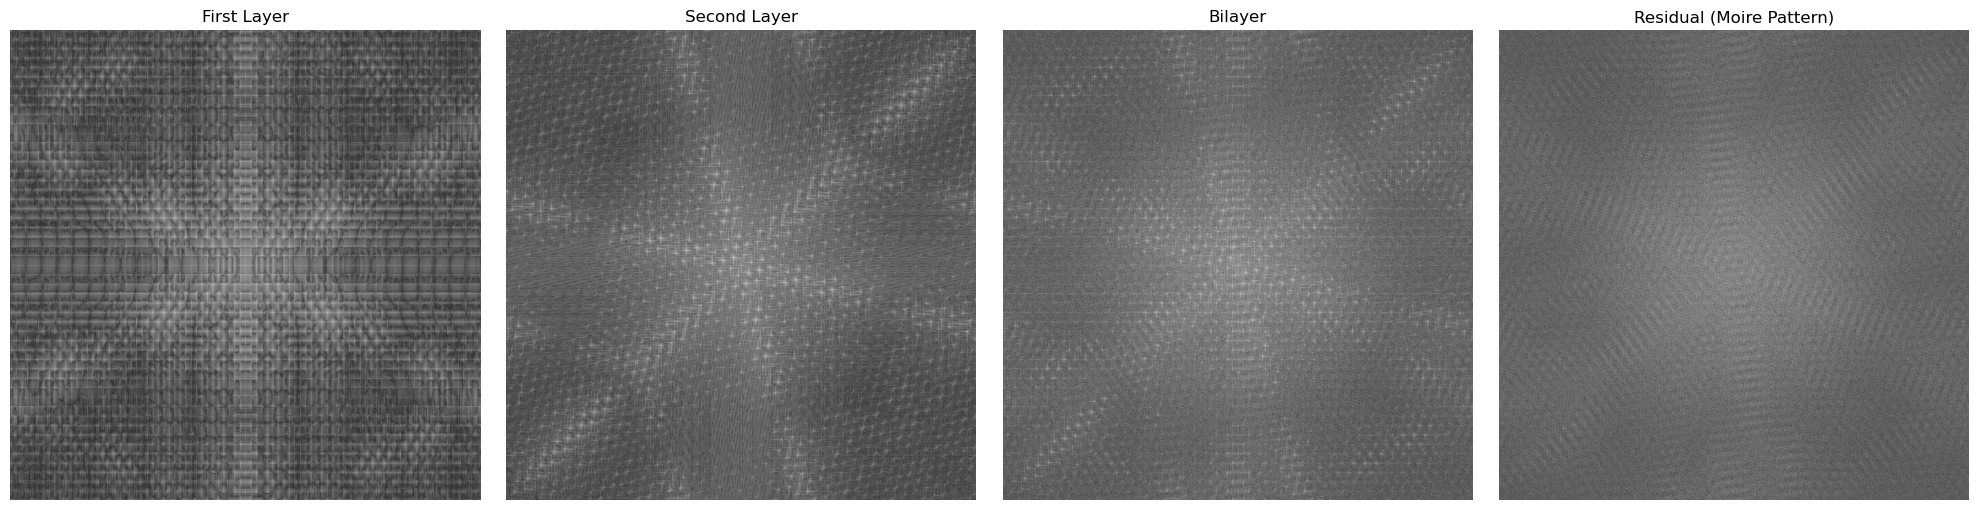
\includegraphics[width=0.95\linewidth]{figures/75degree_fft.png}
        \caption{\textit{continued} (75$^\circ$)}
        \label{fig:moire_75_fft}
    \end{figure}
    \item 90$^\circ$
    \begin{figure}[h]
        \centering
        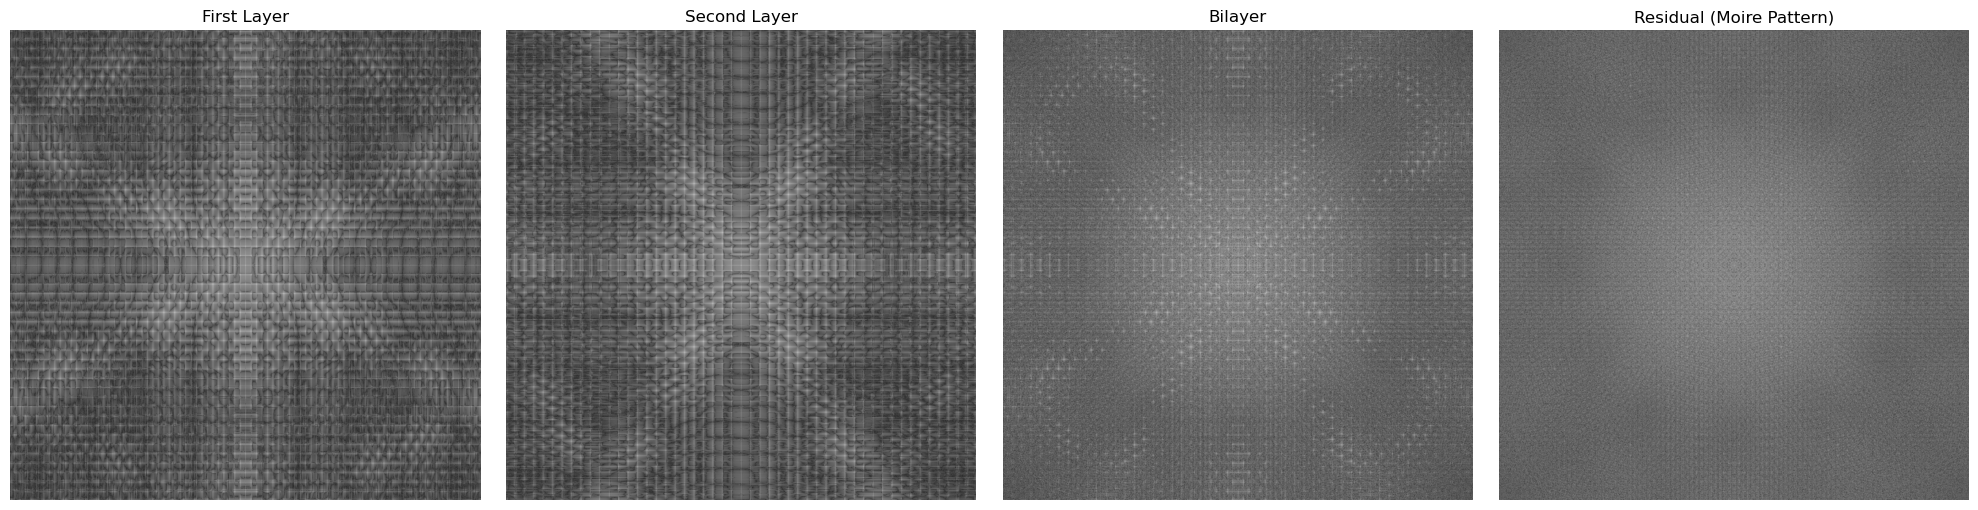
\includegraphics[width=0.95\linewidth]{figures/90degree_fft.png}
        \caption{\textit{continued} (90$^\circ$)}
        \label{fig:moire_90_fft}
    \end{figure}
\end{itemize}
(Note: These spectra should be calculated using complex components to be mathematically correct.)
\clearpage
Secondly, inverse FFT the spectrum of the Moiré pattern $F_{Moire}$ back to real space $f_{Moire}$.

\begin{itemize}
    \item 1$^\circ$
    \begin{figure}[h]
        \centering
        \vspace{-0.5cm}
        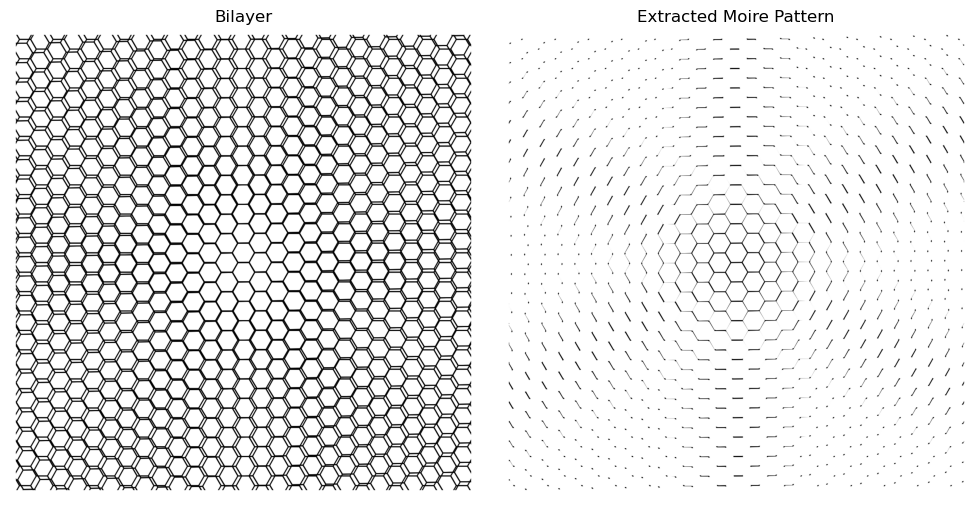
\includegraphics[width=0.65\linewidth]{figures/1degree_moire.png}
        \caption{\textit{left}: The Moiré pattern in the bilayer; \textit{right}: Extracted Moiré pattern(1$^\circ$)}
        \vspace{-0.5cm}
        \label{fig:moire_1_extract}
    \end{figure}
    % \clearpage
    \item 5$^\circ$
    \begin{figure}[h]
        \centering
        \vspace{-0.5cm}
        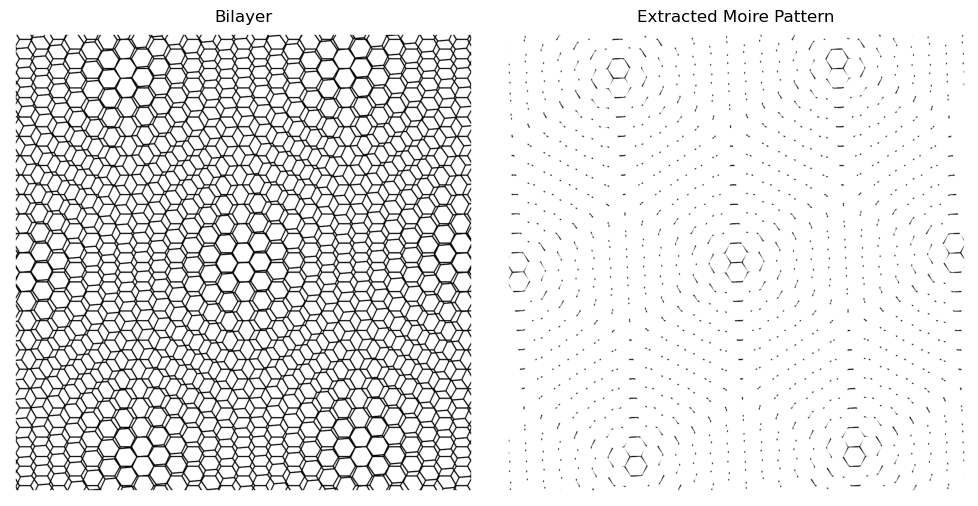
\includegraphics[width=0.65\linewidth]{figures/5degree_moire.png}
        \vspace{-0.5cm}
        \caption{\textit{continued}(5$^\circ$)}
        \label{fig:moire_5_extract}
    \end{figure}
    % \clearpage
    \item 10$^\circ$
    \begin{figure}[h]
        \centering
        \vspace{-0.5cm}
        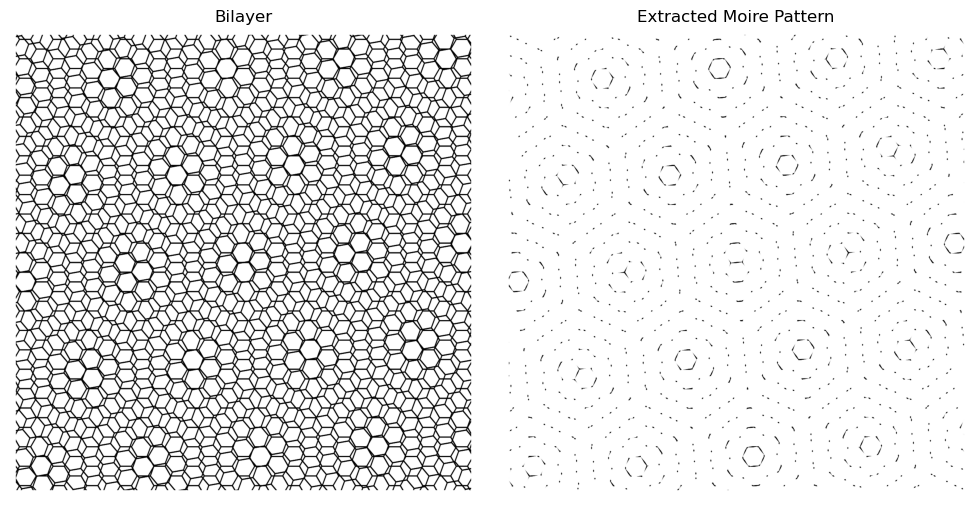
\includegraphics[width=0.65\linewidth]{figures/10degree_moire.png}
        \vspace{-0.5cm}
        \caption{\textit{continued}(10$^\circ$)}
        \label{fig:moire_10_extract}
    \end{figure}
    \clearpage
    \item 15$^\circ$
    \begin{figure}[h]
        \centering
        \vspace{-0.5cm}
        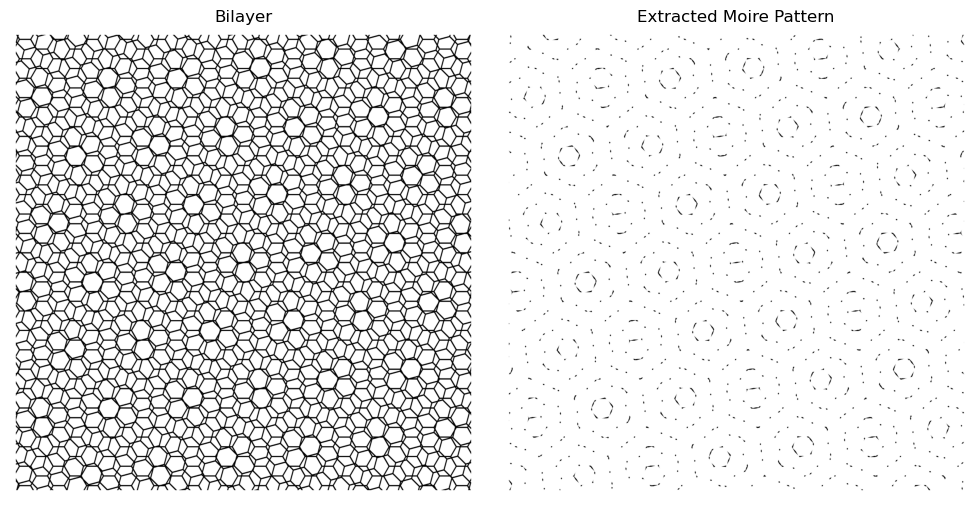
\includegraphics[width=0.65\linewidth]{figures/15degree_moire.png}
        \vspace{-0.5cm}
        \caption{\textit{continued}(15$^\circ$)}
        \label{fig:moire_15_extract}
    \end{figure}
    % \clearpage
    \item 20$^\circ$
    \begin{figure}[h]
        \centering
        \vspace{-0.5cm}
        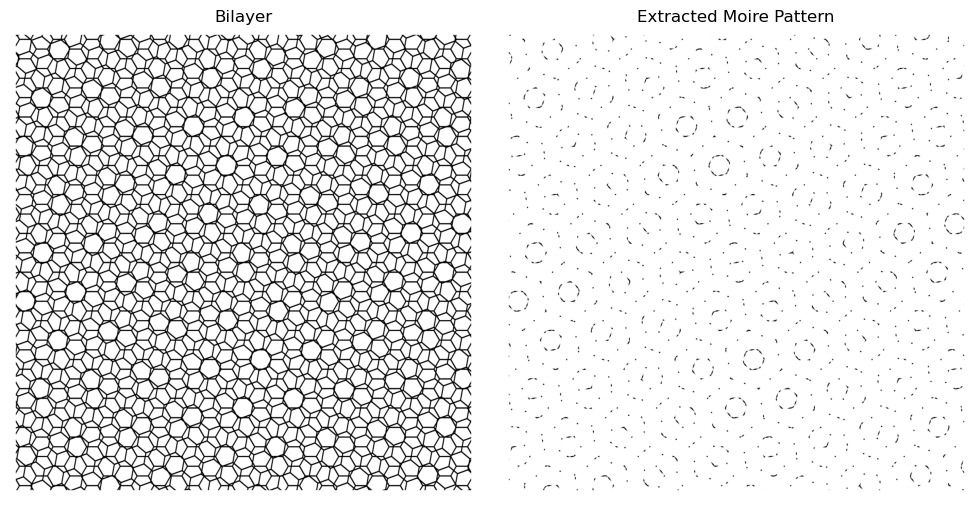
\includegraphics[width=0.65\linewidth]{figures/20degree_moire.png}
        \vspace{-0.5cm}
        \caption{\textit{continued}(20$^\circ$)}
        \label{fig:moire_20_extract}
    \end{figure}
    \item 30$^\circ$
    \begin{figure}[h]
        \centering
        \vspace{-0.5cm}
        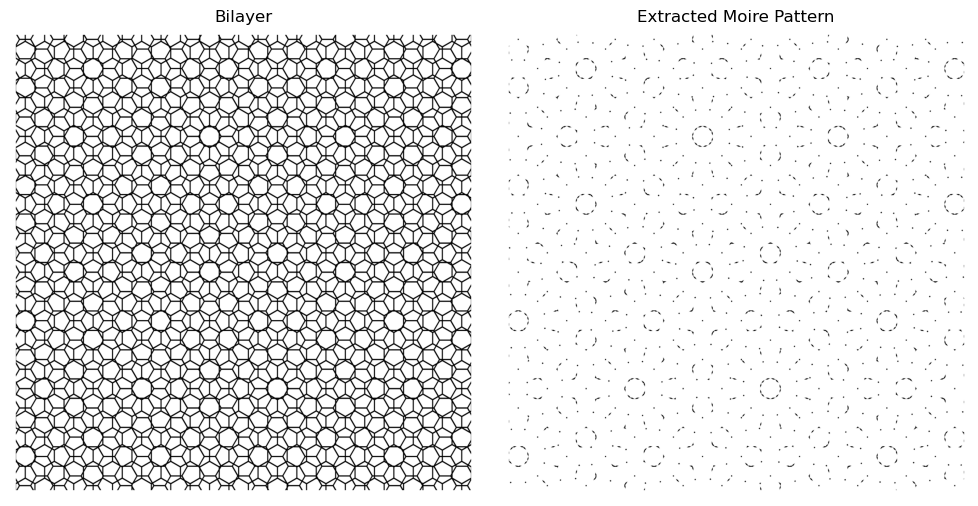
\includegraphics[width=0.65\linewidth]{figures/30degree_moire.png}
        \vspace{-0.5cm}
        \caption{\textit{continued}(30$^\circ$)}
        \label{fig:moire_30_extract}
    \end{figure}
    
    \clearpage
    \item 45$^\circ$
    \begin{figure}[h]
        \centering
        \vspace{-0.5cm}
        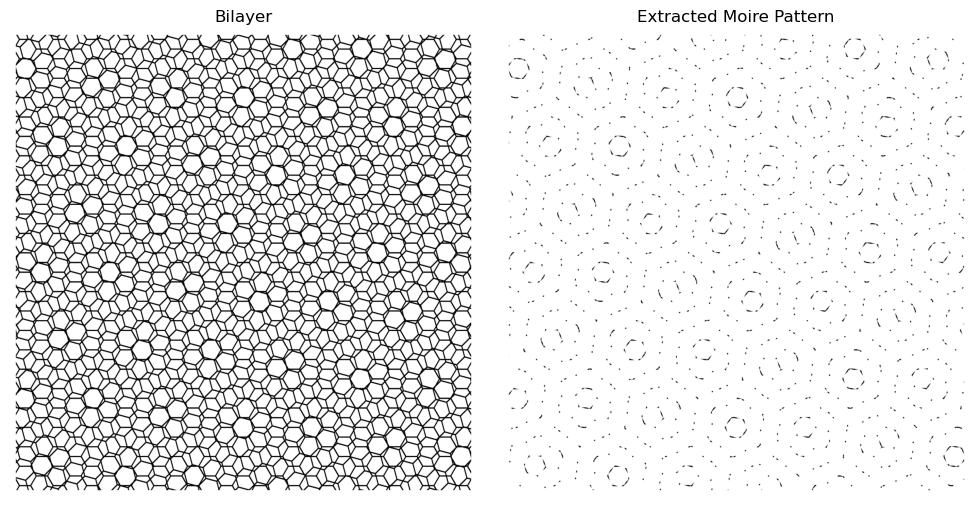
\includegraphics[width=0.65\linewidth]{figures/45degree_moire.png}
        \vspace{-0.5cm}
        \caption{\textit{continued}(45$^\circ$)}
        \label{fig:moire_45_extract}
    \end{figure}
    % \clearpage
    \item 60$^\circ$
    \begin{figure}[h]
        \centering
        \vspace{-0.5cm}
        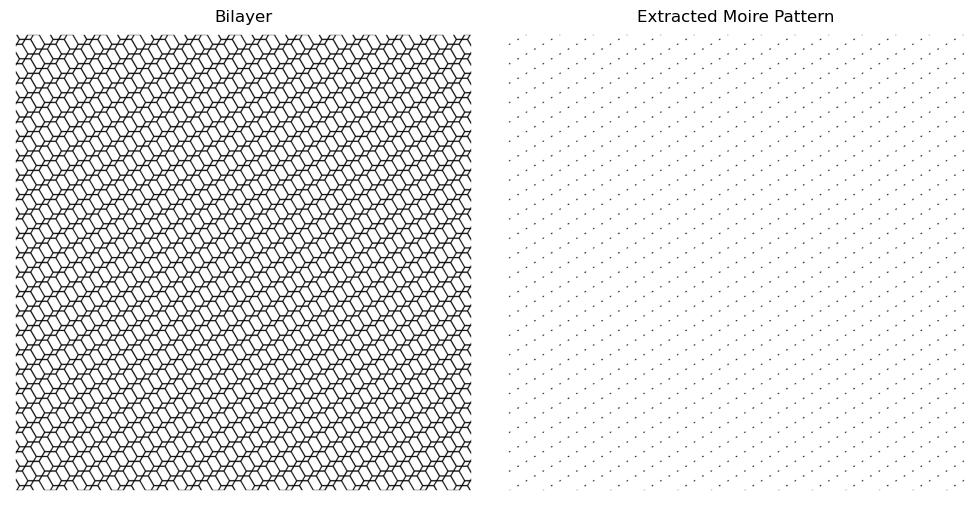
\includegraphics[width=0.65\linewidth]{figures/60degree_moire.png}
        \vspace{-0.5cm}
        \caption{\textit{continued}(60$^\circ$)}
        \label{fig:moire_60_extract}
    \end{figure}
    % \clearpage
    \item 75$^\circ$
    \begin{figure}[h]
        \centering
        \vspace{-0.5cm}
        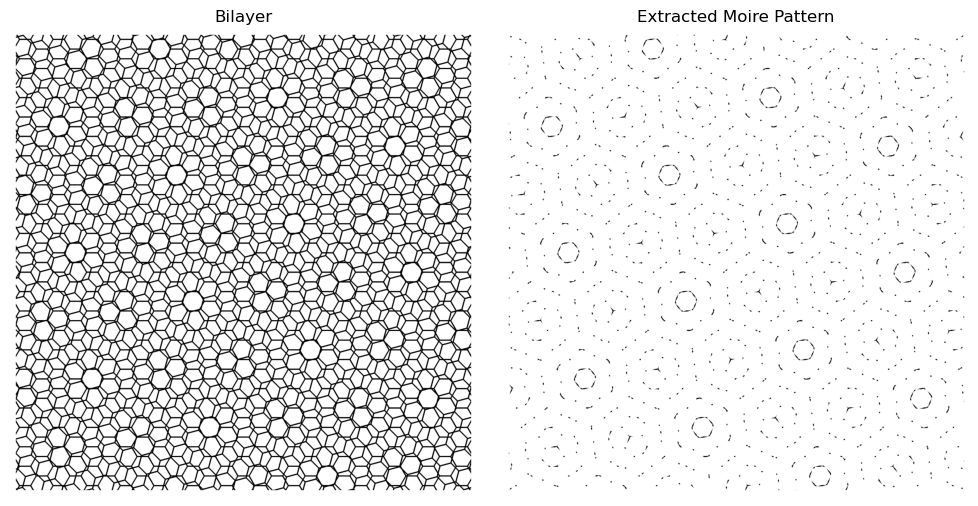
\includegraphics[width=0.65\linewidth]{figures/75degree_moire.png}
        \vspace{-0.5cm}
        \caption{\textit{continued}(75$^\circ$)}
        \label{fig:moire_75_extract}
    \end{figure}
    \clearpage
    \item 90$^\circ$
    \begin{figure}[h]
        \centering
        \vspace{-0.5cm}
        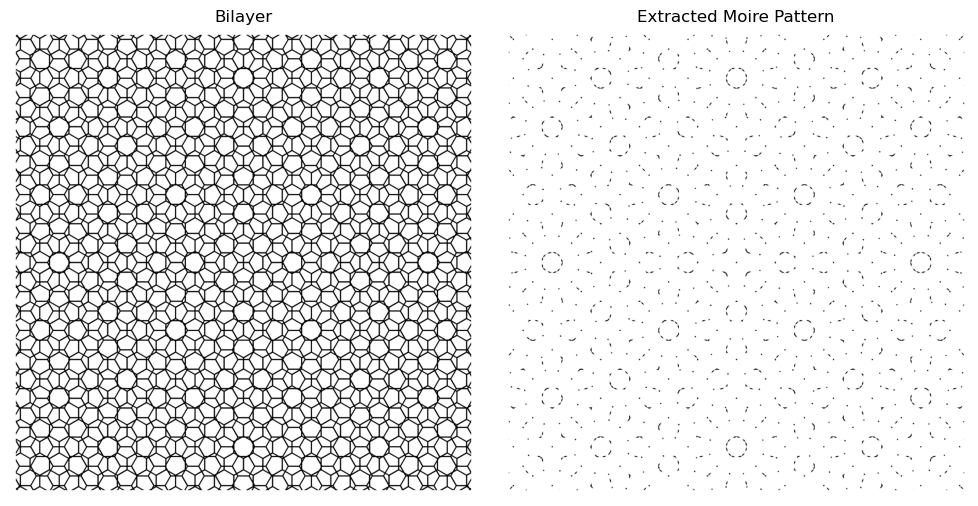
\includegraphics[width=0.65\linewidth]{figures/90degree_moire.png}
        \vspace{-0.5cm}
        \caption{\textit{continued}(90$^\circ$)}
        \label{fig:moire_90_extract}
    \end{figure}
    \end{itemize}
Finally, estimate the periodicity of the extracted Moiré pattern by measuring the number of inter-period pixels and calculating the periodicity by Eq.\ref{eq:moire}. ($a=12$pixels$=$1.42\AA, $a_0=\sqrt{3}a$)
\begin{center}
\begin{tabular}{c|c|c|c}
Twisted angle   &   Measured Periodicity &   Ideal Periodicity   &   Measuring Error\\
($^\circ$)        &              (\AA)     &   (\AA)  &   \%\\
\hline
\hline
1   &   (too large to be measured)       &   57.297  &   -   \\
5   &   10.593  &   11.463  &   7.59\\
10  &   5.612   &   5.737   &   2.18\\
15  &   3.682   &   3.831   &   3.89\\
20  &   2.573   &   2.879   &   8.54\\
30  &   -       &   1.932   &   -   \\
45  &   3.584   &   1.307   &   \textcolor{Gray}{174.21}\\
60  &   -       &   1       &   -   \\
75  &   4.081   &   0.821   &   \textcolor{Gray}{397.07}\\
90  &   -       &   0.707   &   -   
\end{tabular}
\end{center}

As we can see in the table,  if the twisted angle is $5^\circ-20^\circ$, the measured periodicities are nearly the same as the predicted periodicity calculated by Eq.\ref{eq:moire}. However, the measured periodicities seem "saturated" and become immeasurable if the twisted angle is $\theta\geq30^\circ$, here are some possible reasons:
\begin{itemize}
    \item Eq.\ref{eq:moire} is only accurate for small angles.
    \item The periodicities of the actual Moiré patterns are smaller than the bond lengths, inducing \textbf{"aliasing"} (recalling "Nyquist Theorem and Aliasing" last week) when doing FFT. Hence, the extracted Moiré patterns are not fully reconstructed.
    \item When $\theta=60^\circ$, the twisted layer matches the 6-fold symmetry of the graphene, i.e., rotating by $\theta=60^\circ$ brings the lattice back to itself. Therefore, as Fig.\ref{fig:moire_60_extract} shown, no Moiré pattern is extracted.
\end{itemize}

\clearpage
\subsection{Reciprocal Space}\label{subsec:discussion_reciprocal}

\begin{enumerate}
    \item \textbf{Please draw the reciprocal lattice vector G in Fig.\ref{fig:demon_reciprocal}(b) and define the length of G.}\\
    The reciprocal space refers to the wavenumber space, where the unit represents "the number of wave peaks per unit length. $|\mathbf{G}|$ denotes the wavenumber (the number of phases per unit length), while the wavelength represents the spatial period of the wave. The relationship between the two can be referenced in the equation shown in Fig.\ref{fig:demon_reciprocal}(b).
    
    From the calculation results, we can observe the following:
    \begin{itemize}
        \item \textbf{The relationship between $|\mathbf{G}|$ and $\mathbf{a_1}$, $\mathbf{a_2}$:}\\
        As $a_1$ and $a_2$ increase, $|\mathbf{G}|$ decreases, indicating that when the lattice is sparse, the reciprocal lattice becomes denser. A smaller G corresponds to a longer wavelength.
        \item \textbf{The limiting case of wavelength:}\\
        if $a_1=a_2=a$, then $\lambda=a/\sqrt{2}$, meaning that the shortest wavelength in a specific direction is $a/\sqrt{2}$.
    \end{itemize}
    Knowing these results, we can infer the following physical properties:
    \begin{itemize}
        \item \textbf{Material structure analysis:}\\
        Given $\lambda$, we can derive $|\mathbf{G}|$, then infer $a_1$, $a_2$ to determine whether the crystal structure is uniform.
        \item \textbf{Directional dependence:}\\
        Since $\lambda$ varies when $a1\neq a2$, it indicates that $\lambda$ is direction-dependent. This allows us to analyze whether a crystal exhibits stronger or weaker properties (e.g., conductivity, optical properties) in certain directions.
    \end{itemize}
    \item \textbf{Use the relationship ($\mathbf{b_i \cdot a_i} =2\pi \delta_{ij}$ where $\delta_{ij}=1$ if $i=j$ and $\delta_{ij}=0$ if $i\neq j$) to obtain the reciprocal lattice vectors of graphene and again use python to generate the reciprocal lattice point of graphene. Find the diffraction patterns of graphene from a website and define the reciprocal lattice vectors. Compare these obtained vectors with your results.}\\
    Each bright spot corresponds to a reciprocal lattice point, matching the blue points in the Python-generated plot. The structure also exhibits hexagonal symmetry, but it reflects density and directional properties. Brighter spots (center and some key points) represent lower-order reciprocal lattice points, while farther spots are higher-order with reduced intensity.


    Comparison of Fig.\ref{fig:result_2_2_11} with our generated plot Fig.\ref{fig:result_2_2_9}
    \begin{itemize}
        \item The reciprocal lattice we plotted consists of a hexagonally symmetric pattern formed by a parallelogram grid.
        \item Fig.\ref{fig:result_2_2_11} exhibits the same structure but without the grid boundaries drawn
        \item The central point corresponds to the reciprocal space origin(0,0).
        \item The alignment and density of the points in the experimental diffraction pattern match the points in our Python-generated plot.
    \end{itemize}
    \clearpage
    \item \textbf{Use the lattice points and the reciprocal lattice vectors you obtained from Python to check if reciprocal lattice points can be mapped out by the set of reciprocal lattice vectors that yield plane waves with the periodicity of a given Bravais lattice.}\\
    \begin{itemize}
        \item \textbf{Distribution of Reciprocal Lattice Points:}\\
        In Fig.\ref{fig:result_2_2_9}, blue dots represent the reciprocal lattice points, while orange dashed lines indicate the unit cell of the reciprocal lattice. The red and green arrows correspond to the reciprocal lattice vectors $\mathbf{b}_1$ and $\mathbf{b}_2$, respectively. The reciprocal lattice points generated by Python exhibit a hexagonal arrangement, which aligns with theoretical calculations and confirms the hexagonal symmetry of the reciprocal lattice.
        \item \textbf{Periodicity of Plane Waves:}\\
        The mathematical form of the plane wave is:
        \begin{equation}
            \psi(r) = e^{i\mathbf{G}\cdot\mathbf{r}}
        \end{equation}
        Here is the source code to generate the plane wave:
        \begin{enumerate}
            \item Initialize reciprocal vectors $\mathbf{b}_1$ and $\mathbf{b}_2$. The two reciprocal lattice vectors of graphene are manually defined to describe the periodicity in reciprocal space.
            \begin{figure}[h]
                \centering
                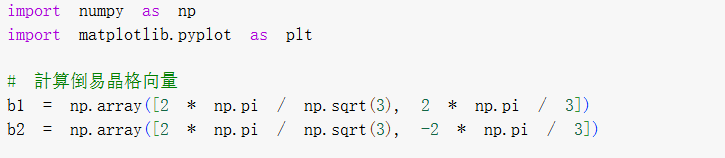
\includegraphics[width=0.7\linewidth]{figures/discussion_2_3_1.png}
                \caption{Initialize reciprocal vectors}
                \label{fig:disc_2_3_1}
            \end{figure}
            \item Define a function of plane wave
            \begin{figure}[h]
                \centering
                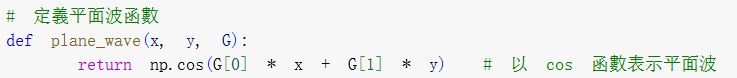
\includegraphics[width=0.7\linewidth]{figures/discussion_2_3_2.png}
                \caption{Function of plane wave}
                \label{fig:disc_2_3_2}
            \end{figure}
             \item Create a mesh grid and the corresponding plane wave (choose $\mathbf{b}_1$) 
             \begin{figure}[h]
                 \centering
                 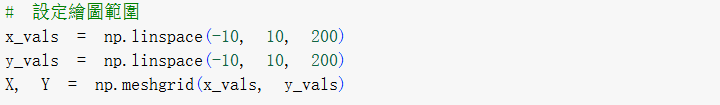
\includegraphics[width=0.7\linewidth]{figures/discussion_2_3_3.png}\\
                 \includegraphics[width=0.7\linewidth]{figures/discussion_2_3_4.png}
                 \caption{Create a mesh grid and the corresponding plane wave}
                 \label{fig:disc_2_3_3}
             \end{figure}
             \clearpage
             \item Make a plot of the plane wave
             \begin{figure}[h]
                 \centering
                 \includegraphics[width=0.7\linewidth]{figures/discussion_2_3_5.png}
                 \caption{Plot plane wave}
                 \label{fig:disc_2_3_5}
             \end{figure}
        \end{enumerate}
    \begin{figure}[h]
        \centering
        \includegraphics[width=0.7\linewidth]{figures/plane_wave.png}
        \caption{The plane wave corresponding to $\mathbf{b}_1$}
        \label{fig:plane_wave}
    \end{figure}
    The generated contour plot (Fig.\ref{fig:plane_wave}) shows that the spacing between wavefronts matches the reciprocal lattice vectors, indicating that the plane wave indeed exhibits the periodicity of the reciprocal lattice, thereby verifying the correctness of the theory.
    \end{itemize}
\end{enumerate}


\clearpage
\section{Conclusion}\label{sec:conclusion}
\hfill

In this experiment, we explored the representations of graphene in real and reciprocal space and analyzed the relationships between lattice vectors, reciprocal lattice vectors, and diffraction patterns. Through Python simulations, we generated both the graphene lattice structure and its corresponding reciprocal lattice. Additionally, we investigated the Moiré patterns produced by twisted bilayer graphene. We examined the relationship between their periodicity and twist angle, confirming that as the twist angle decreases, the Moiré pattern’s periodicity increases.

The reciprocal lattice structure obtained from our Python simulation exhibits hexagonal symmetry, which aligns with the theoretical model. By applying the reciprocal lattice condition, we computed the reciprocal lattice vectors and verified the periodicity of the system. Furthermore, the simulated reciprocal lattice points closely match the diffraction patterns from external references. We also analyzed how reciprocal lattice vectors affect the periodicity of plane waves. Using Python, we created contour plots of wave vectors corresponding to reciprocal lattice points. The results demonstrate that these plane waves exhibit periodicity consistent with the Bravais lattice.


\section{Work division}\label{sec:work}
% \hfill

\begin{itemize}
    \item 洪瑜: Reciprocal space, Report
    \item 黃巧涵: Plane wave, Report
    \item 洪懌平: Graphene and Moiré patterns, Report
\end{itemize}

\begin{figure}[h]
    \centering
    \includegraphics[width=0.30\linewidth]{figures/hyu.jpg}
    \includegraphics[width=0.30\linewidth]{figures/hch.jpg}
    \includegraphics[width=0.30\linewidth]{figures/hyp.jpg}
    \caption{洪瑜(\textit{left}), 黃巧涵(\textit{middle}), and 洪懌平(\textit{right})}
    \label{fig:work}
\end{figure}

% \clearpage
\section{Source codes of these exercises}

\begin{itemize}
    \item FFT of a square pulse: \url{https://github.com/hyp0515/exp_phy_ii/blob/main/mar18/squre_pulse.ipynb}
    \item Generating graphene's lattice structure: \url{https://github.com/hyp0515/exp_phy_ii/blob/main/mar18/graphene.ipynb}
    \item Generating a twisted bilayer graphene Moiré pattern: \url{https://github.com/hyp0515/exp_phy_ii/blob/main/mar18/moire_pattern.ipynb}
    \item Reciprocal lattice and plane wave: \url{https://colab.research.google.com/drive/1tj_p0CpQVOKVBAET_oL-Sx_tk9qLaxlg?usp=sharing}
\end{itemize}

\clearpage
\section{Reference}\label{sec:reference}
% \hfill

\begin{itemize}
    \item [1]: \url{https://shorturl.at/Xephu}
    \item [2]: \url{https://shorturl.at/SMwrn}
    \item [3]: \url{https://shorturl.at/0Qxmq}
\end{itemize}


\end{CJK}
\end{document}
